% !TeX root = ../tfg.tex
% !TeX encoding = utf8
%
%*******************************************************
% Capítulo 10. Detección OOD
%*******************************************************

\chapter{Detección OOD}\label{cap:deteccion-ood}

% Patrón: tabla o figura -> análisis; discusión global al final.
% Fuente: results_ood/faseC_K144 (= faseC_2026-10-20 más la fila de STOOD-X con K = 144; 17 métodos,
% 9 conjuntos). Modelo: Swin-S (mismo checkpoint
% que la \cref{tab:modelos}). Métricas definidas en el \cref{cap:ood-metricas}; clase positiva: OOD.
% Además de los nueve conjuntos, las 27 celdas de corrupciones sintéticas (9 corrupciones x niveles 1, 3
% y 5; \cref{sec:ood-corrupciones}).
\pendiente{introducción del capítulo: modelo, 17 métodos (13 de OpenOOD y cuatro configuraciones de STOOD-X: 100\,\% y 87,5\,\% con $K = 500$, $K_c$ y $K = 144$, \cref{sec:stoodx-seleccion-k}), nueve conjuntos (\cref{tab:diseno-ood}) y métricas (\cref{sec:auroc,sec:fpr95,sec:ccr}); IC por \emph{bootstrap} (\cref{sec:bootstrap})}

% Diferencia de exactitud del Swin-S en el test ID: 0,9688 (results_fase1) frente a 0,9687 en la
% evaluación OOD (features/completo/id_test.npz; también 0,96870 en el nivel 0 de results_corrupciones).
% Las predicciones coinciden en 12.617 de 12.618 imágenes. Única diferencia:
% Glandulas_no_neoplasicas/30113155_017249_016353_000224.png (clase real Glandulas_no_neoplasicas):
% la fase 1 acierta y la evaluación OOD predice Gleason_3; las dos probabilidades más altas están casi
% empatadas (fase 1: 0,4371 frente a 0,4337; OOD: 0,4391 frente a 0,4321).
% Entornos según los ficheros: fase 1 (fase1_predicciones.py, results_fase1/predicciones_info.json,
% script_fase1.sh) y fase A (results_ood/faseA_*/config.json) usan el mismo entorno fastai_env_ood
% (torch 2.8.0+cu128) y la misma GPU (RTX 2080 Ti). Lo que cambia es la ruta de inferencia: la fase 1
% carga el learner exportado (.pkl) con learn.get_preds, que «usa la precisión mixta del learner»
% (results_fase1/resumen.md); la fase A carga el state dict (.pth) en fp32 con el transform de
% my_evauator_openood.py. La exactitud medida al entrenar (resultados.txt de param4: fastai_env,
% torch 1.12.1, TITAN Xp) es 0,96870, igual que la de la evaluación OOD.
\revisar{el autor atribuye la diferencia a un cambio de entorno (versión de PyTorch y hardware), pero según los ficheros la fase 1 y la extracción OOD comparten entorno y GPU; la diferencia está en la ruta de inferencia (learner con precisión mixta frente a state dict en fp32). Confirmar la causa antes de redactar la nota}
\pendiente{nota al pie sobre la diferencia de exactitud por cambio de entorno}

\revisar{la tabla principal de las notas (\texttt{tabla\_principal\_ood.tex}) se divide en una tabla por bloque; las tablas de AUPR van al \cref{ap:aupr}}

\begin{figure}[tbp]
  \centering
  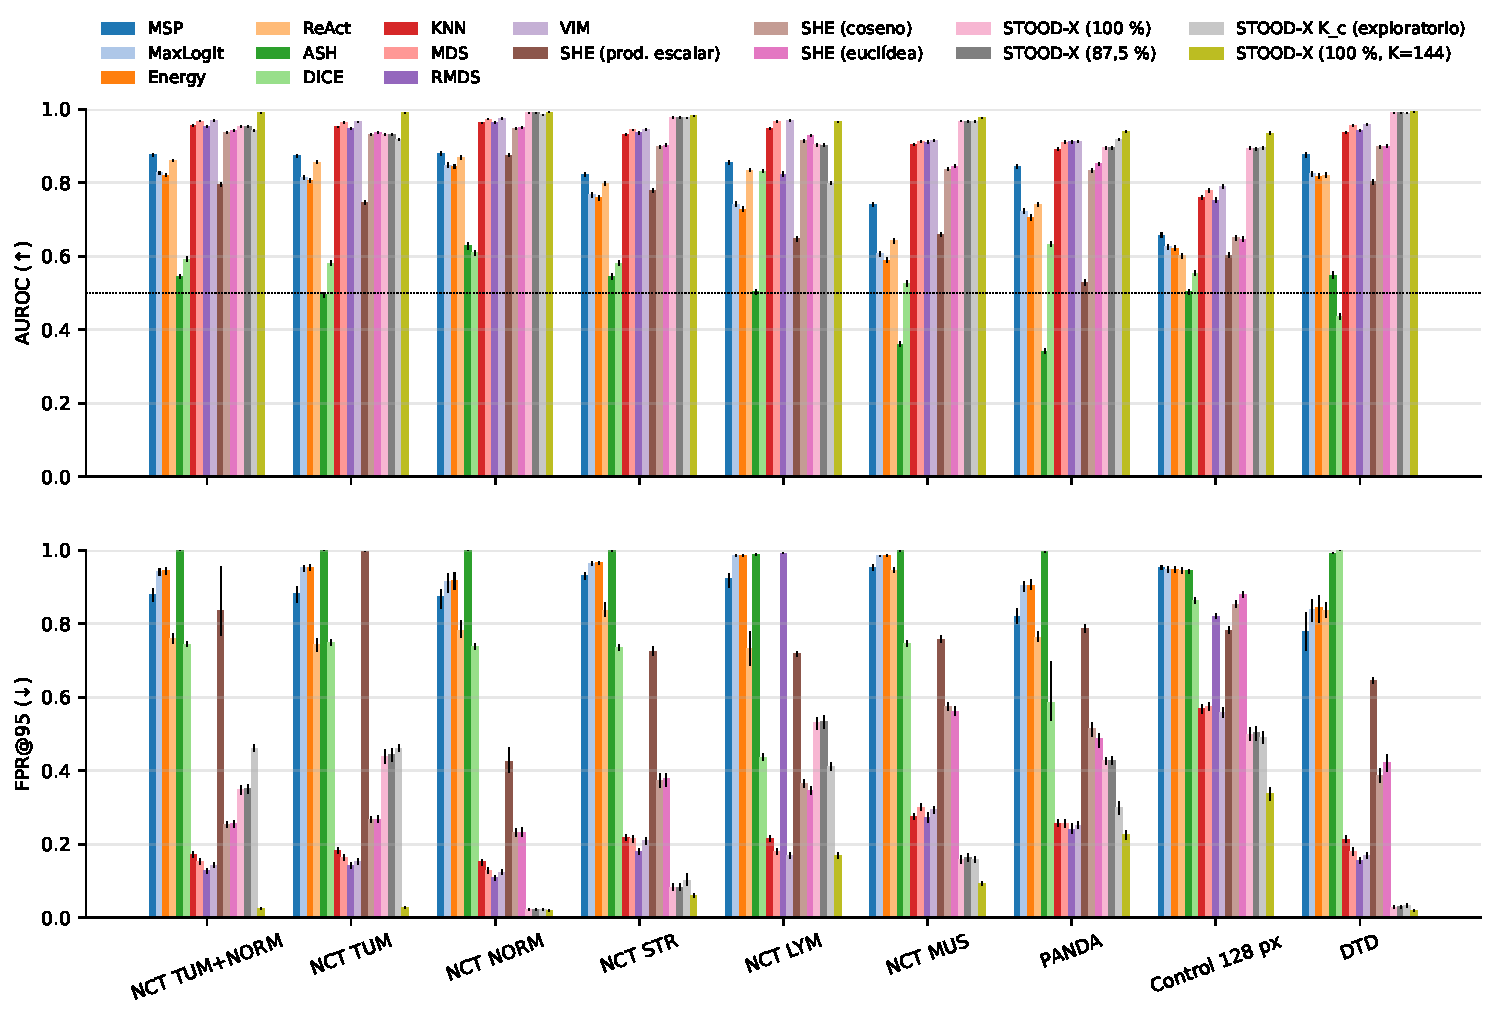
\includegraphics[width=\textwidth]{img/cap10/fig1_auroc_fpr95.pdf}
  \caption{AUROC (arriba; más alto es mejor) y FPR@95 (abajo; más bajo es mejor) de los 17 métodos en los nueve conjuntos, con IC del 95\,\% por \emph{bootstrap}. Visión global de la comparación.}
  \label{fig:ood-global}
\end{figure}

\section{Near-OOD principal}\label{sec:ood-near}

Los resultados muestran una separación clara entre familias de métodos. Los métodos que operan sobre el espacio de características (ViM, MDS, KNN, RMDS y STOOD-X) superan de forma sistemática a los basados únicamente en los logits, en todos los conjuntos evaluados. En el near-OOD principal (NCT-CRC TUM + NORM), los primeros alcanzan un AUROC de entre 0,953 y 0,969, frente a 0,821--0,876 de MSP, MaxLogit y Energy. La diferencia es aún mayor en el punto de trabajo: el FPR@95 baja de 0,879 (MSP) a valores entre 0,128 y 0,173, y el CCR@FPR5 sube de 0,118 a más de 0,82. Esto indica que el vector de características de 768 dimensiones contiene información sobre la pertenencia a la distribución que se pierde al proyectarlo sobre los 14 logits. \revisar{en ConvNeXt-S (espacio M), MSP (0,954) supera a MDS (0,949) y solo RMDS (0,960) queda por encima en TUM+NORM: matizar como propio del Swin (\cref{ap:convnext})}
\revisar{«de forma sistemática [...] en todos los conjuntos»: RMDS queda por debajo de MSP en LYM (AUROC 0,824 frente a 0,854, \cref{tab:ood-control-interno})}
\revisar{el rango de AUROC (0,953--0,969), el de FPR@95 (0,128--0,173) y el CCR@FPR5 (más de 0,82) valen para ViM, MDS, KNN, RMDS y STOOD-X con $K = 500$ (salvo FPR@95 y CCR@FPR5 de STOOD-X: 0,349 y 0,646); STOOD-X con $K = 144$ queda por encima de los tres rangos (AUROC 0,991, FPR@95 0,026, CCR@FPR5 0,951)}

% Generado por scripts/generar_tablas.py a partir de results_ood/faseC_K144/tabla_principal.csv. No editar a mano.
\begin{table}
\centering
\footnotesize
\setlength{\tabcolsep}{4pt}
\caption{Near-OOD principal (\nctcrc, TUM+NORM): \AUROC y \CCRn{5} (más alto es mejor) y \FPRn{95} (más bajo es mejor) de los 17 métodos. IC del 95\,\% por \emph{bootstrap} (1.000 remuestreos estratificados, semilla 0). Clase positiva: OOD. En negrita, el mejor valor entre los métodos no exploratorios. $^{a}$ASH reduce la exactitud ID al 68{,}3\,\%. $^{\dagger}$Variante exploratoria ($K_c=\min(500,\lfloor n_c/2\rfloor)$), propuesta tras ver datos OOD; no es el método principal. $^{\ddagger}$100\,\% de las características y $K=144$, elegido solo con la validación ID (\cref{sec:stoodx-seleccion-k}); el resto de filas de \stoodx usan $K=500$, el valor del artículo.}
\label{tab:ood-near}
\begin{tabular}{lccc}
\toprule
Método & \AUROC $\uparrow$ [IC 95\,\%] & \FPRn{95} $\downarrow$ [IC 95\,\%] & \CCRn{5} $\uparrow$ \\
\midrule
\multicolumn{4}{@{}l}{\textit{Basados en logits}} \\
MSP & 0{,}876 [0{,}872; 0{,}879] & 0{,}879 [0{,}861; 0{,}895] & 0{,}118 \\
MaxLogit & 0{,}828 [0{,}823; 0{,}832] & 0{,}942 [0{,}932; 0{,}952] & 0{,}056 \\
Energy & 0{,}821 [0{,}817; 0{,}825] & 0{,}944 [0{,}935; 0{,}952] & 0{,}054 \\
\midrule
\multicolumn{4}{@{}l}{\textit{Modificación de activaciones}} \\
ReAct & 0{,}861 [0{,}857; 0{,}864] & 0{,}760 [0{,}745; 0{,}773] & 0{,}238 \\
ASH$^{a}$ & 0{,}546 [0{,}540; 0{,}551] & 0{,}999 [0{,}998; 1{,}000] & 0{,}001 \\
DICE & 0{,}592 [0{,}585; 0{,}598] & 0{,}744 [0{,}737; 0{,}753] & 0{,}254 \\
\midrule
\multicolumn{4}{@{}l}{\textit{Características y distancias}} \\
KNN & 0{,}956 [0{,}954; 0{,}958] & 0{,}173 [0{,}165; 0{,}180] & 0{,}825 \\
MDS & 0{,}968 [0{,}966; 0{,}969] & 0{,}152 [0{,}144; 0{,}160] & 0{,}844 \\
RMDS & 0{,}954 [0{,}951; 0{,}956] & 0{,}128 [0{,}121; 0{,}134] & 0{,}868 \\
ViM & 0{,}969 [0{,}968; 0{,}971] & 0{,}143 [0{,}136; 0{,}150] & 0{,}853 \\
SHE (prod.\ escalar) & 0{,}795 [0{,}790; 0{,}800] & 0{,}837 [0{,}768; 0{,}955] & 0{,}162 \\
SHE (coseno) & 0{,}938 [0{,}935; 0{,}940] & 0{,}255 [0{,}246; 0{,}263] & 0{,}743 \\
SHE (euclídea) & 0{,}942 [0{,}940; 0{,}944] & 0{,}255 [0{,}246; 0{,}265] & 0{,}742 \\
\midrule
\multicolumn{4}{@{}l}{\textit{STOOD-X}} \\
STOOD-X (100\,\%) & 0{,}953 [0{,}951; 0{,}955] & 0{,}349 [0{,}335; 0{,}360] & 0{,}646 \\
STOOD-X ($K=144$)$^{\ddagger}$ & \textbf{0{,}991} [0{,}990; 0{,}992] & \textbf{0{,}026} [0{,}023; 0{,}028] & \textbf{0{,}951} \\
STOOD-X (87,5\,\%) & 0{,}953 [0{,}951; 0{,}955] & 0{,}352 [0{,}338; 0{,}363] & 0{,}644 \\
STOOD-X $K_c$$^{\dagger}$ & 0{,}943 [0{,}941; 0{,}945] & 0{,}461 [0{,}453; 0{,}471] & 0{,}535 \\
\bottomrule
\end{tabular}
\end{table}


\textbf{Near-OOD principal.} Entre los métodos con su configuración por defecto, ViM (0,969 [0,968; 0,971]) y MDS (0,968) obtienen el mejor AUROC, mientras que RMDS logra el mejor FPR@95 (0,128) y el mejor CCR@FPR5 (0,868), con un AUROC significativamente inferior (0,954; \cref{tab:ood-bootstrap-rmds}). Ambos resultados no son contradictorios: el AUROC resume la separación en todos los umbrales, mientras que FPR@95 y CCR@FPR5 evalúan la zona de umbral exigente, que es la relevante en un contexto clínico (\cref{fig:ood-roc}). Con el umbral que deja pasar solo el 5\,\% de las imágenes de colon, RMDS acepta y clasifica correctamente el 86,8\,\% del test ID, frente a un máximo posible de 96,9\,\%. No obstante, RMDS presenta un fallo marcado en la clase LYM (FPR@95 $= 0{,}992$; CCR@FPR5 $= 0{,}008$): una parte de los linfocitos de colon recibe puntuaciones superiores a las de las propias imágenes ID, por lo que ningún umbral permite rechazarlos sin descartar casi todo el ID.
\revisar{añadidas las referencias a la \cref{tab:ood-bootstrap-rmds} y a la \cref{fig:ood-roc}}
Con $K = 144$, elegido solo con datos ID (\cref{sec:stoodx-seleccion-k}), \stoodx supera a todos ellos en las tres métricas: \AUROC 0,991 [0,990; 0,992], \FPRn{95} 0,026 [0,023; 0,028] y \CCRn{5} 0,951. Su ventaja sobre RMDS en \AUROC es de 0,037 [0,035; 0,040] (\cref{tab:ood-bootstrap-rmds}), mientras que con $K = 500$ ambos métodos eran indistinguibles.
\revisar{añadido «Entre los métodos con su configuración por defecto» y la frase sobre $K = 144$ (redactada por el agente a petición del autor): con $K = 144$, ViM, MDS y RMDS dejan de ser los mejores en TUM+NORM}

% Generado por scripts/generar_tablas.py a partir de results_ood/faseC_K144/bootstrap_pareado_rmds.csv. No editar a mano.
\begin{table}
\centering
\footnotesize
\caption{\emph{Bootstrap} pareado (1.000 remuestreos, semilla 0) de la diferencia \AUROC(RMDS) $-$ \AUROC(método) en el near-OOD principal (TUM+NORM); RMDS es el método de referencia, por lo que no tiene fila propia. Diferencia positiva: RMDS es mejor. $p<0{,}001$: ninguna réplica cruzó el cero. $^{a}$, $^{\dagger}$: como en \cref{tab:ood-near}.}
\label{tab:ood-bootstrap-rmds}
\begin{tabular}{lccc}
\toprule
Método & Diferencia & IC 95\,\% & $p$ \\
\midrule
MSP & +0{,}078 & [0{,}075; 0{,}081] & $<0{,}001$ \\
MaxLogit & +0{,}126 & [0{,}122; 0{,}130] & $<0{,}001$ \\
Energy & +0{,}133 & [0{,}129; 0{,}136] & $<0{,}001$ \\
ReAct & +0{,}093 & [0{,}090; 0{,}096] & $<0{,}001$ \\
ASH$^{a}$ & +0{,}408 & [0{,}402; 0{,}414] & $<0{,}001$ \\
DICE & +0{,}362 & [0{,}356; 0{,}369] & $<0{,}001$ \\
KNN & $-$0{,}003 & [-0{,}004; -0{,}001] & 0{,}002 \\
MDS & $-$0{,}014 & [-0{,}015; -0{,}012] & $<0{,}001$ \\
ViM & $-$0{,}016 & [-0{,}017; -0{,}014] & $<0{,}001$ \\
SHE (prod.\ escalar) & +0{,}159 & [0{,}155; 0{,}163] & $<0{,}001$ \\
SHE (coseno) & +0{,}016 & [0{,}014; 0{,}018] & $<0{,}001$ \\
SHE (euclídea) & +0{,}012 & [0{,}010; 0{,}014] & $<0{,}001$ \\
STOOD-X (100\,\%) & +0{,}000 & [-0{,}002; 0{,}003] & 0{,}752 \\
STOOD-X (87,5\,\%) & +0{,}001 & [-0{,}001; 0{,}003] & 0{,}556 \\
STOOD-X $K_c$$^{\dagger}$ & +0{,}011 & [0{,}008; 0{,}013] & $<0{,}001$ \\
STOOD-X ($K=144$)$^{\ddagger}$ & $-$0{,}037 & [-0{,}040; -0{,}035] & $<0{,}001$ \\
\bottomrule
\end{tabular}
\end{table}


\begin{figure}[tbp]
  \centering
  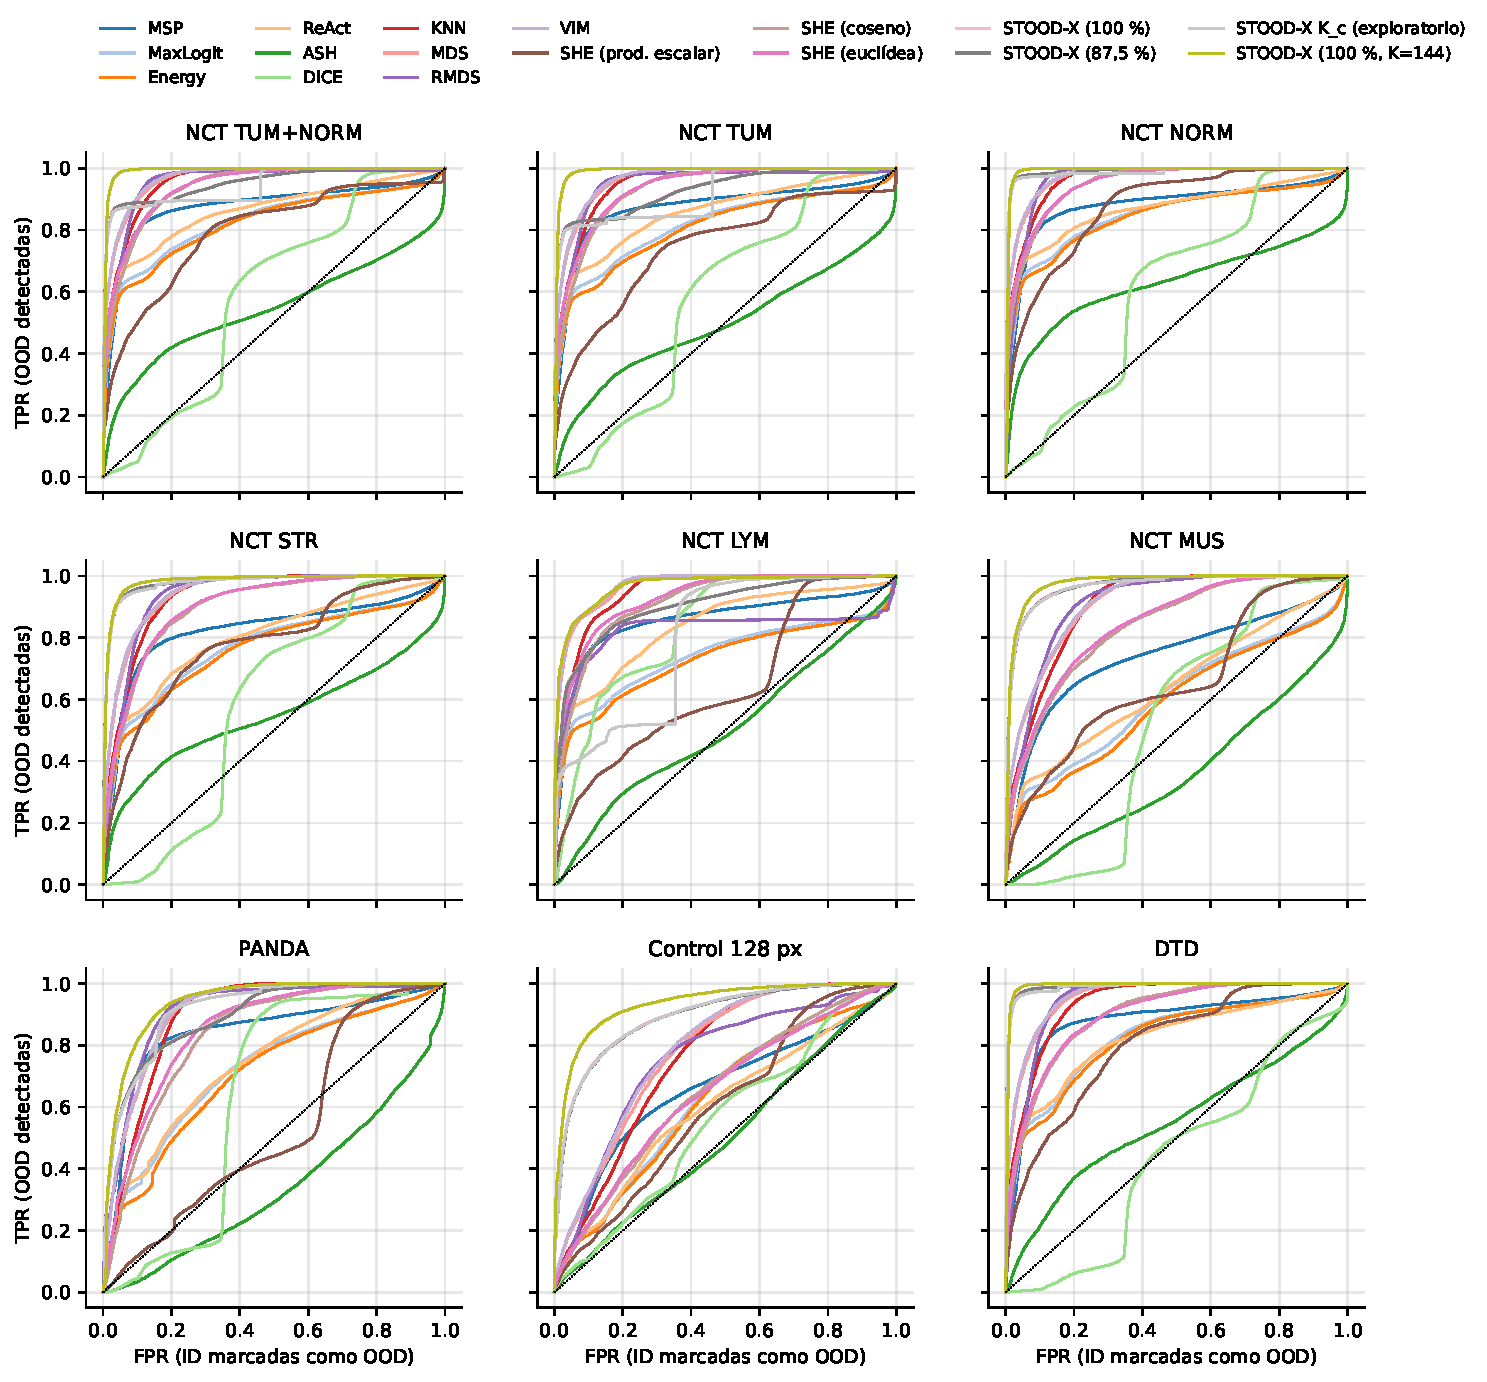
\includegraphics[width=\textwidth]{img/cap10/fig2_curvas_roc.pdf}
  \caption{Curvas ROC (TPR sobre OOD frente a FPR sobre ID) de todos los métodos, un panel por conjunto. Permiten ver dónde se separan los métodos: la zona de FPR baja frente al AUROC global explica por qué RMDS es el mejor en FPR@95 y no en AUROC.}
  \label{fig:ood-roc}
\end{figure}

% Cifras de la \cref{tab:ood-bootstrap-rmds}: RMDS - ViM = -0,016 [-0,017; -0,014]; RMDS - MDS =
% -0,014; RMDS - KNN = -0,003 [-0,004; -0,001] (p = 0,002); RMDS - STOOD-X 100 % = +0,000
% [-0,002; +0,003] (p = 0,75); RMDS - STOOD-X K = 144 = -0,037 [-0,040; -0,035] (p < 0,001). Los IC de FPR@95 de RMDS [0,121; 0,134] y ViM [0,136; 0,150] no se
% solapan, pero no se hizo bootstrap pareado para FPR@95.

\section{Control interno: centro frente a tejido}\label{sec:ood-control-interno}

% Generado por scripts/generar_tablas.py a partir de results_ood/faseC_K144/tabla_principal.csv. No editar a mano.
\begin{table}
\centering
\scriptsize
\setlength{\tabcolsep}{2.5pt}
\caption{Control interno con las clases de \nctcrc: tejido glandular de colon (TUM y NORM) frente a tejidos análogos a clases ID (STR, LYM y MUS). \AUROC (más alto es mejor) y \FPRn{95} (más bajo es mejor).}
\label{tab:ood-control-interno}
\begin{tabular*}{\linewidth}{@{\extracolsep{\fill}}lcccccccccccc}
\toprule
& \multicolumn{6}{c}{\AUROC $\uparrow$} & \multicolumn{6}{c}{\FPRn{95} $\downarrow$} \\
\cmidrule(lr){2-7}\cmidrule(lr){8-13}
Método & TUM & NORM & STR & LYM & MUS & Media & TUM & NORM & STR & LYM & MUS & Media \\
\midrule
\multicolumn{13}{@{}l}{\textit{Basados en logits}} \\
MSP & 0{,}873 & 0{,}880 & 0{,}823 & 0{,}854 & 0{,}740 & 0{,}834 & 0{,}882 & 0{,}875 & 0{,}931 & 0{,}923 & 0{,}954 & 0{,}913 \\
MaxLogit & 0{,}815 & 0{,}848 & 0{,}767 & 0{,}741 & 0{,}607 & 0{,}756 & 0{,}952 & 0{,}916 & 0{,}965 & 0{,}985 & 0{,}985 & 0{,}961 \\
Energy & 0{,}807 & 0{,}844 & 0{,}759 & 0{,}727 & 0{,}589 & 0{,}745 & 0{,}952 & 0{,}918 & 0{,}966 & 0{,}986 & 0{,}986 & 0{,}962 \\
\textit{Media del grupo} & 0{,}832 & 0{,}857 & 0{,}783 & 0{,}774 & 0{,}646 & 0{,}778 & 0{,}929 & 0{,}903 & 0{,}954 & 0{,}965 & 0{,}975 & 0{,}945 \\
\midrule
\multicolumn{13}{@{}l}{\textit{Modificación de activaciones}} \\
ReAct & 0{,}856 & 0{,}868 & 0{,}798 & 0{,}835 & 0{,}643 & 0{,}800 & 0{,}743 & 0{,}783 & 0{,}836 & 0{,}734 & 0{,}946 & 0{,}808 \\
ASH$^{a}$ & 0{,}496 & 0{,}628 & 0{,}544 & 0{,}504 & 0{,}361 & 0{,}506 & 0{,}999 & 0{,}999 & 0{,}998 & 0{,}989 & 0{,}999 & 0{,}997 \\
DICE & 0{,}581 & 0{,}609 & 0{,}581 & 0{,}831 & 0{,}525 & 0{,}626 & 0{,}750 & 0{,}738 & 0{,}734 & 0{,}436 & 0{,}746 & 0{,}681 \\
\textit{Media del grupo} & 0{,}644 & 0{,}702 & 0{,}641 & 0{,}723 & 0{,}510 & 0{,}644 & 0{,}831 & 0{,}840 & 0{,}856 & 0{,}720 & 0{,}897 & 0{,}829 \\
\midrule
\multicolumn{13}{@{}l}{\textit{Características y distancias}} \\
KNN & 0{,}952 & 0{,}963 & 0{,}932 & 0{,}948 & 0{,}904 & 0{,}940 & 0{,}183 & 0{,}152 & 0{,}219 & 0{,}216 & 0{,}275 & 0{,}209 \\
MDS & 0{,}964 & 0{,}973 & 0{,}944 & 0{,}967 & 0{,}912 & 0{,}952 & 0{,}164 & 0{,}129 & 0{,}215 & 0{,}181 & 0{,}301 & 0{,}198 \\
RMDS & 0{,}947 & 0{,}964 & 0{,}935 & 0{,}824 & 0{,}911 & 0{,}916 & 0{,}142 & 0{,}109 & 0{,}180 & 0{,}992 & 0{,}272 & 0{,}339 \\
ViM & 0{,}966 & 0{,}975 & 0{,}946 & 0{,}969 & 0{,}915 & 0{,}954 & 0{,}154 & 0{,}124 & 0{,}209 & 0{,}170 & 0{,}293 & 0{,}190 \\
SHE (prod.\ escalar) & 0{,}746 & 0{,}875 & 0{,}780 & 0{,}647 & 0{,}660 & 0{,}741 & 0{,}997 & 0{,}426 & 0{,}725 & 0{,}718 & 0{,}757 & 0{,}725 \\
SHE (coseno) & 0{,}931 & 0{,}948 & 0{,}898 & 0{,}914 & 0{,}837 & 0{,}906 & 0{,}267 & 0{,}233 & 0{,}373 & 0{,}365 & 0{,}574 & 0{,}363 \\
SHE (euclídea) & 0{,}937 & 0{,}950 & 0{,}902 & 0{,}928 & 0{,}845 & 0{,}912 & 0{,}267 & 0{,}231 & 0{,}378 & 0{,}346 & 0{,}562 & 0{,}357 \\
\textit{Media del grupo} & 0{,}921 & 0{,}950 & 0{,}905 & 0{,}885 & 0{,}855 & 0{,}903 & 0{,}310 & 0{,}201 & 0{,}329 & 0{,}427 & 0{,}434 & 0{,}340 \\
\midrule
\multicolumn{13}{@{}l}{\textit{STOOD-X}} \\
STOOD-X (100\,\%) & 0{,}931 & 0{,}990 & 0{,}978 & 0{,}903 & 0{,}968 & 0{,}954 & 0{,}440 & 0{,}022 & 0{,}083 & 0{,}531 & 0{,}159 & 0{,}247 \\
STOOD-X ($K=144$)$^{\ddagger}$ & 0{,}990 & 0{,}992 & 0{,}982 & 0{,}966 & 0{,}977 & 0{,}981 & 0{,}029 & 0{,}020 & 0{,}061 & 0{,}170 & 0{,}093 & 0{,}074 \\
STOOD-X (87,5\,\%) & 0{,}930 & 0{,}990 & 0{,}978 & 0{,}903 & 0{,}967 & 0{,}954 & 0{,}444 & 0{,}022 & 0{,}082 & 0{,}533 & 0{,}164 & 0{,}249 \\
STOOD-X $K_c$$^{\dagger}$ & 0{,}917 & 0{,}985 & 0{,}977 & 0{,}799 & 0{,}966 & 0{,}929 & 0{,}461 & 0{,}023 & 0{,}101 & 0{,}411 & 0{,}158 & 0{,}231 \\
\textit{Media del grupo} & 0{,}942 & 0{,}989 & 0{,}979 & 0{,}893 & 0{,}969 & 0{,}954 & 0{,}343 & 0{,}022 & 0{,}082 & 0{,}411 & 0{,}144 & 0{,}200 \\
\bottomrule
\end{tabular*}

\smallskip
\parbox{\linewidth}{\scriptsize Clase positiva: OOD. Media: media aritmética de los cinco conjuntos. Media del grupo: media aritmética de todas las filas del grupo. $^{a}$ASH reduce la exactitud ID al 68{,}3\,\%. $^{\dagger}$Variante exploratoria ($K_c=\min(500,\lfloor n_c/2\rfloor)$), propuesta tras ver datos OOD; no es el método principal. $^{\ddagger}$100\,\% de las características y $K=144$, elegido solo con la validación ID (\cref{sec:stoodx-seleccion-k}); el resto de filas de \stoodx usan $K=500$, el valor del artículo.}
\end{table}


Los resultados muestran que el principal motivo por el que una imagen se detecta como OOD es que procede de condiciones de adquisición distintas (otro centro y láminas no vistas). 
Con MDS, TUM (0,964), NORM (0,973) y LYM (0,967) obtienen los valores de AUROC más altos. El caso de LYM es el más revelador: pese a corresponder a un tipo de tejido presente en 
la próstata, se detecta con la misma capacidad que el tejido de colon. STR (0,944) y MUS (0,912) resultan algo más difíciles de detectar, lo que indica que la similitud con las 
clases ID influye en parte, aunque los valores siguen siendo altos. Este resultado es coherente con lo señalado por Yang et al.~\cite{yang2024}: los detectores OOD tienden a ser 
más sensibles al desplazamiento de covariables que al cambio semántico.

\begin{figure}[tbp]
  \centering
  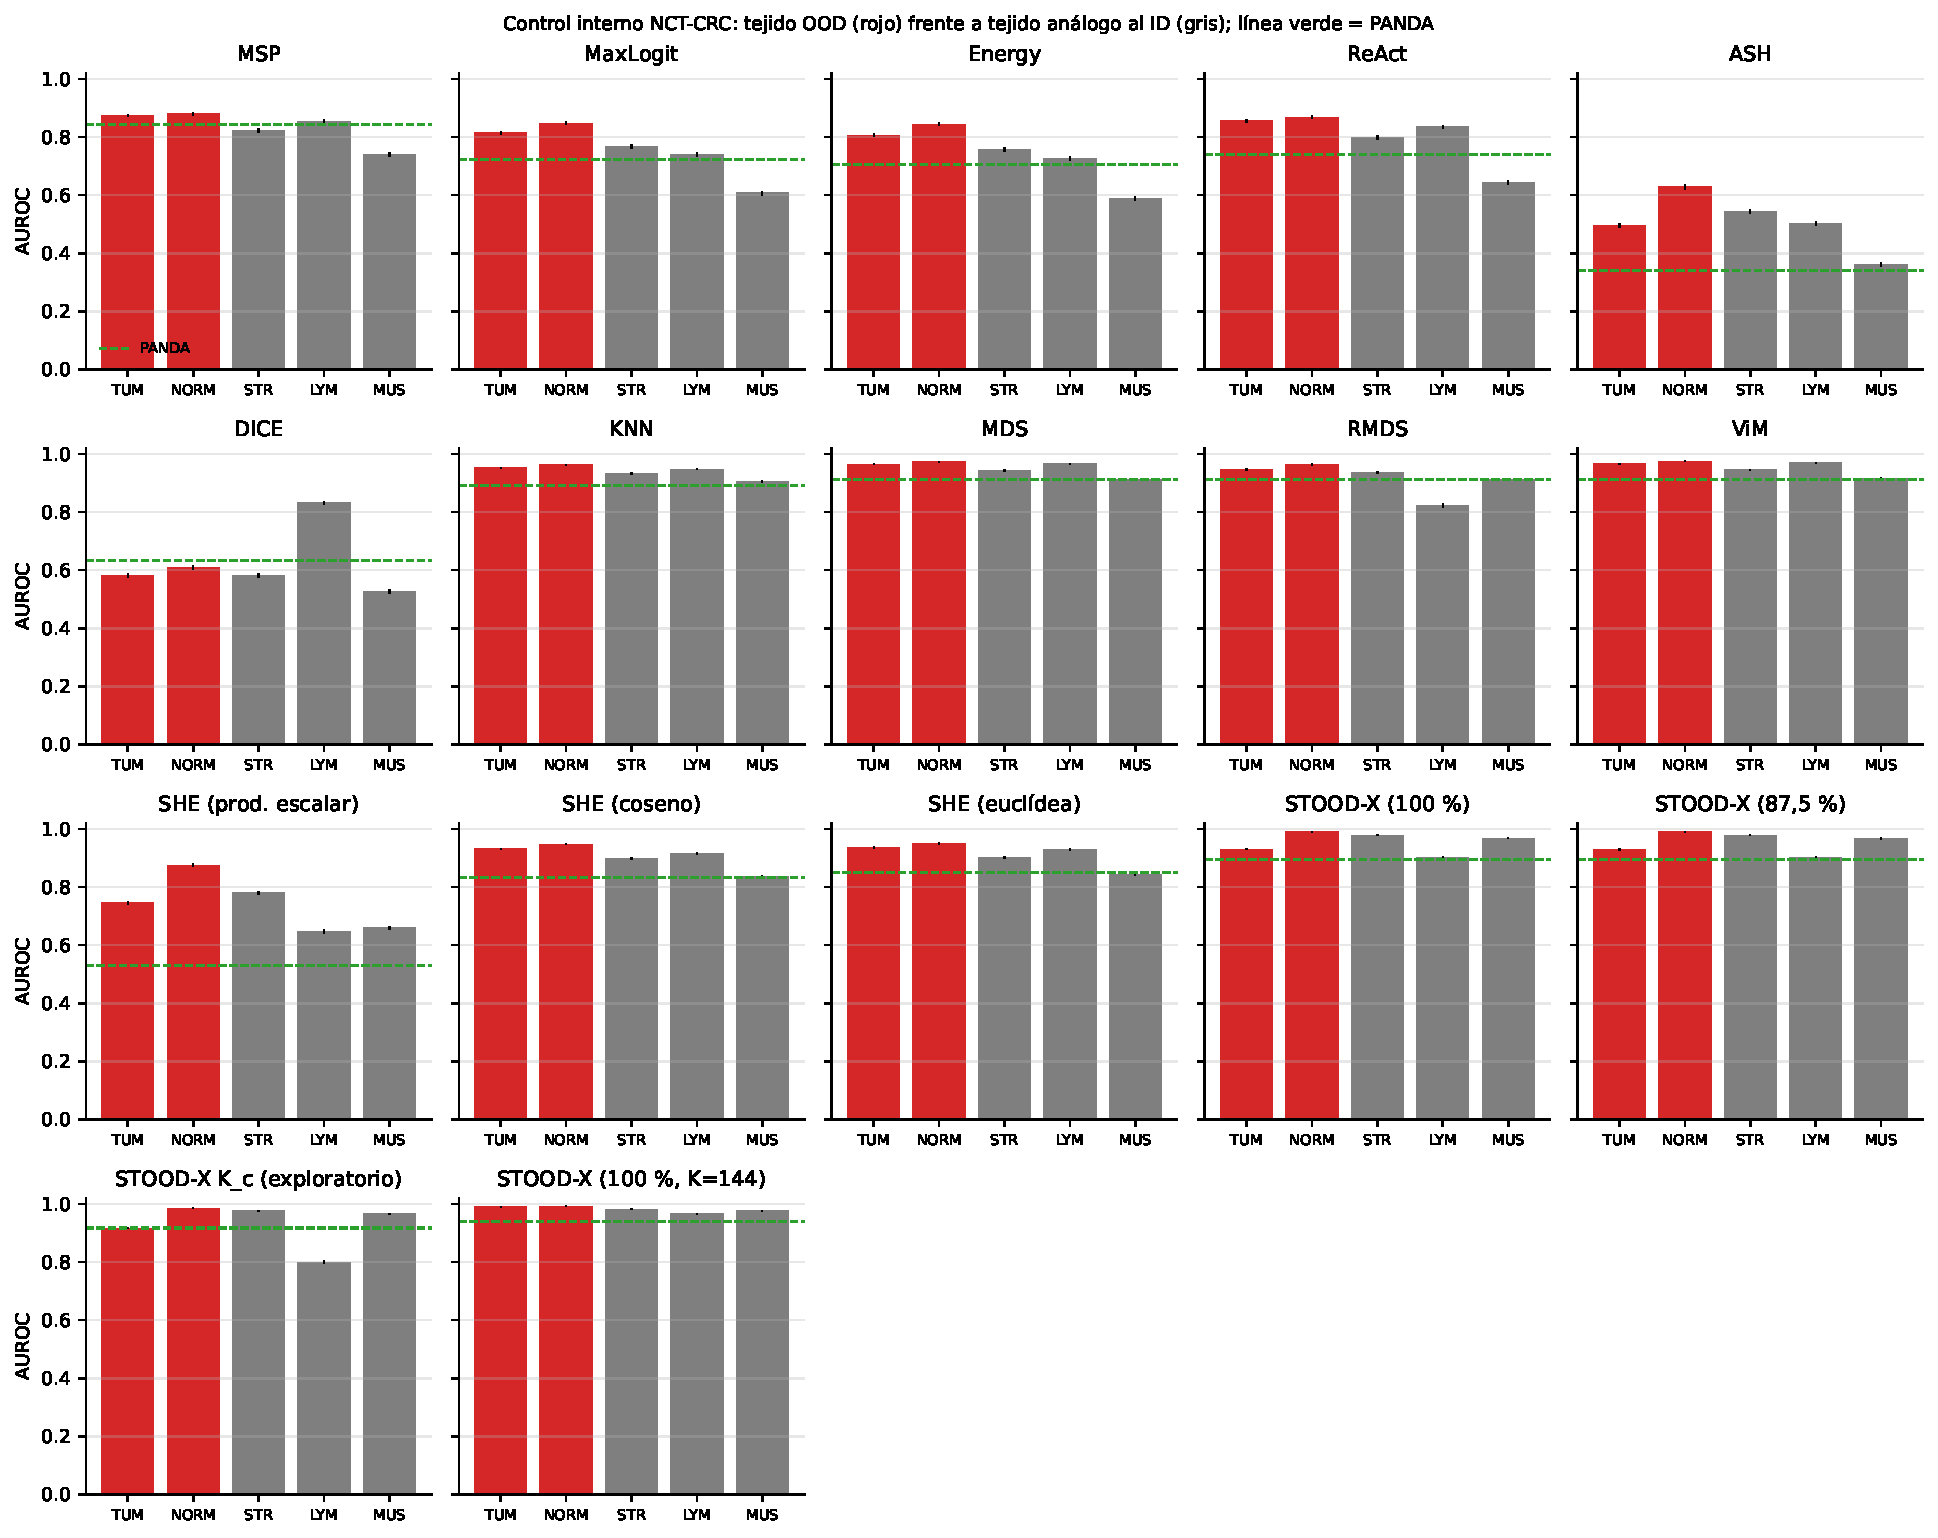
\includegraphics[width=\textwidth]{img/cap10/fig5_control_interno_nct.pdf}
  \caption{AUROC por clase de NCT-CRC (TUM y NORM en rojo; STR, LYM y MUS en gris) para cada método, con PANDA como línea de referencia. Control interno del centro frente al tejido: si las clases afines se detectan casi igual que TUM y NORM, el detector responde al centro.}
  \label{fig:ood-control-interno}
\end{figure}

% Cifras adicionales: en STOOD-X con K = 500, STR (0,978) y MUS (0,968) se detectan más que TUM (0,931).
% Con K = 144 el orden cambia: TUM 0,990, NORM 0,992, STR 0,982, LYM 0,966, MUS 0,977. En los
% métodos de logits la diferencia es mayor (MSP: 0,87-0,88 en TUM/NORM frente a 0,74 en MUS), con
% LYM (0,854) cerca de TUM/NORM. La conclusión se mantiene sin la lámina de cada parche
% (\cref{tab:fuga-control-interno}).

\section{PANDA: cambio de centro y de escala}\label{sec:ood-panda}

Respecto a PANDA, la comparación con el control debe interpretarse con especial cuidado, ya que sus imágenes presentan más diferencias que el mero reescalado. Además de proceder de otros centros, las teselas se extrajeron del nivel de menor resolución de las imágenes originales, con un aumento mucho menor, de modo que cada una abarca una región de tejido muy superior a los 112\,$\mu$m de los parches ID; además, contienen mucho más fondo blanco (63\,\% frente a 21\,\%). Los métodos de distancia detectan PANDA (AUROC $\approx 0{,}91$) mejor que el control ($\approx 0{,}77$--$0{,}79$), pero esta diferencia no puede atribuirse solo al cambio de centro, ya que se combina con los cambios de escala y de contenido de fondo. En STOOD-X, ambos AUROC coinciden (0,895 y 0,894) y su puntuación no distingue PANDA del control (AUROC 0,475 [0,467; 0,482]). Sin embargo, cerca de un tercio de las imágenes de ambos conjuntos alcanza el valor extremo del estadístico (\cref{obs:u-empates}), por lo que esta coincidencia refleja la pérdida de capacidad de ordenación por saturación más que una sensibilidad específica a la resolución. \revisar{reforzar: con ConvNeXt-S (espacio M), menos saturado (22,0\,\% en TUM+NORM y 2,6\,\% en el control, frente a 66,3\,\% y 19,0\,\% en el Swin), STOOD-X sí distingue PANDA del control (0,803 [0,797; 0,809]); \cref{tab:convnext-stoodx}}
\revisar{estas cifras de STOOD-X son con $K = 500$. Con $K = 144$, PANDA (0,939) y el control (0,935) siguen casi igualados (\cref{fig:ood-panda-control}) con menos saturación que en TUM+NORM (30\,\% de PANDA y 39\,\% del control saturados, \cref{tab:stoodx-saturacion-k144}), así que la explicación por saturación no basta para $K = 144$; el AUROC de PANDA frente al control (0,475) no se ha calculado con $K = 144$} Excluir las 291 teselas sin tejido no modifica ninguna de estas conclusiones. Aislar el efecto del centro requeriría extraer las imágenes de PANDA a la misma escala que los datos ID, lo que queda como trabajo futuro.

% Generado por scripts/generar_tablas.py a partir de results_ood/faseC_K144/tabla_principal.csv. No editar a mano.
\begin{table}
\centering
\scriptsize
\setlength{\tabcolsep}{3pt}
\caption{PANDA (próstata de otros centros, adquirida a una escala mucho menor) frente al control de resolución (las mismas imágenes del test ID reducidas a 128\,px). \AUROC (más alto es mejor) y \FPRn{95} (más bajo es mejor). Diferencia: \AUROC de PANDA menos \AUROC del control. IC del 95\,\% por \emph{bootstrap} (1.000 remuestreos estratificados, semilla 0). Clase positiva: OOD. $^{a}$ASH reduce la exactitud ID al 68{,}3\,\%. $^{\dagger}$Variante exploratoria ($K_c=\min(500,\lfloor n_c/2\rfloor)$), propuesta tras ver datos OOD; no es el método principal. $^{\ddagger}$100\,\% de las características y $K=144$, elegido solo con la validación ID (\cref{sec:stoodx-seleccion-k}); el resto de filas de \stoodx usan $K=500$, el valor del artículo.}
\label{tab:ood-panda-control}
\begin{tabular}{lccccc}
\toprule
& \multicolumn{3}{c}{\AUROC $\uparrow$ [IC 95\,\%]} & \multicolumn{2}{c}{\FPRn{95} $\downarrow$} \\
\cmidrule(lr){2-4}\cmidrule(lr){5-6}
Método & PANDA & Control 128\,px & Diferencia & PANDA & Control \\
\midrule
\multicolumn{6}{@{}l}{\textit{Basados en logits}} \\
MSP & 0{,}843 [0{,}838; 0{,}849] & 0{,}657 [0{,}650; 0{,}664] & +0{,}186 & 0{,}821 & 0{,}953 \\
MaxLogit & 0{,}723 [0{,}716; 0{,}730] & 0{,}626 [0{,}619; 0{,}633] & +0{,}097 & 0{,}904 & 0{,}948 \\
Energy & 0{,}706 [0{,}698; 0{,}713] & 0{,}622 [0{,}615; 0{,}629] & +0{,}084 & 0{,}905 & 0{,}948 \\
\midrule
\multicolumn{6}{@{}l}{\textit{Modificación de activaciones}} \\
ReAct & 0{,}741 [0{,}734; 0{,}747] & 0{,}602 [0{,}594; 0{,}609] & +0{,}140 & 0{,}764 & 0{,}945 \\
ASH$^{a}$ & 0{,}341 [0{,}334; 0{,}348] & 0{,}503 [0{,}496; 0{,}510] & -0{,}162 & 0{,}996 & 0{,}944 \\
DICE & 0{,}633 [0{,}626; 0{,}639] & 0{,}554 [0{,}547; 0{,}561] & +0{,}079 & 0{,}586 & 0{,}864 \\
\midrule
\multicolumn{6}{@{}l}{\textit{Características y distancias}} \\
KNN & 0{,}892 [0{,}887; 0{,}896] & 0{,}760 [0{,}754; 0{,}765] & +0{,}132 & 0{,}256 & 0{,}569 \\
MDS & 0{,}911 [0{,}907; 0{,}914] & 0{,}780 [0{,}774; 0{,}785] & +0{,}131 & 0{,}257 & 0{,}575 \\
RMDS & 0{,}912 [0{,}908; 0{,}916] & 0{,}753 [0{,}747; 0{,}759] & +0{,}159 & 0{,}241 & 0{,}821 \\
ViM & 0{,}912 [0{,}909; 0{,}916] & 0{,}789 [0{,}784; 0{,}794] & +0{,}123 & 0{,}252 & 0{,}558 \\
SHE (prod.\ escalar) & 0{,}530 [0{,}522; 0{,}537] & 0{,}603 [0{,}596; 0{,}610] & -0{,}073 & 0{,}787 & 0{,}783 \\
SHE (coseno) & 0{,}834 [0{,}829; 0{,}839] & 0{,}651 [0{,}644; 0{,}657] & +0{,}184 & 0{,}514 & 0{,}854 \\
SHE (euclídea) & 0{,}851 [0{,}847; 0{,}856] & 0{,}646 [0{,}639; 0{,}653] & +0{,}205 & 0{,}488 & 0{,}881 \\
\midrule
\multicolumn{6}{@{}l}{\textit{STOOD-X}} \\
STOOD-X (100\,\%) & 0{,}895 [0{,}891; 0{,}899] & 0{,}894 [0{,}890; 0{,}898] & +0{,}001 & 0{,}427 & 0{,}497 \\
STOOD-X ($K=144$)$^{\ddagger}$ & 0{,}939 [0{,}936; 0{,}942] & 0{,}935 [0{,}932; 0{,}938] & +0{,}004 & 0{,}226 & 0{,}339 \\
STOOD-X (87,5\,\%) & 0{,}895 [0{,}891; 0{,}899] & 0{,}893 [0{,}889; 0{,}897] & +0{,}002 & 0{,}428 & 0{,}505 \\
STOOD-X $K_c$$^{\dagger}$ & 0{,}917 [0{,}914; 0{,}921] & 0{,}895 [0{,}891; 0{,}898] & +0{,}023 & 0{,}300 & 0{,}490 \\
\bottomrule
\end{tabular}
\end{table}


\begin{figure}[tbp]
  \centering
  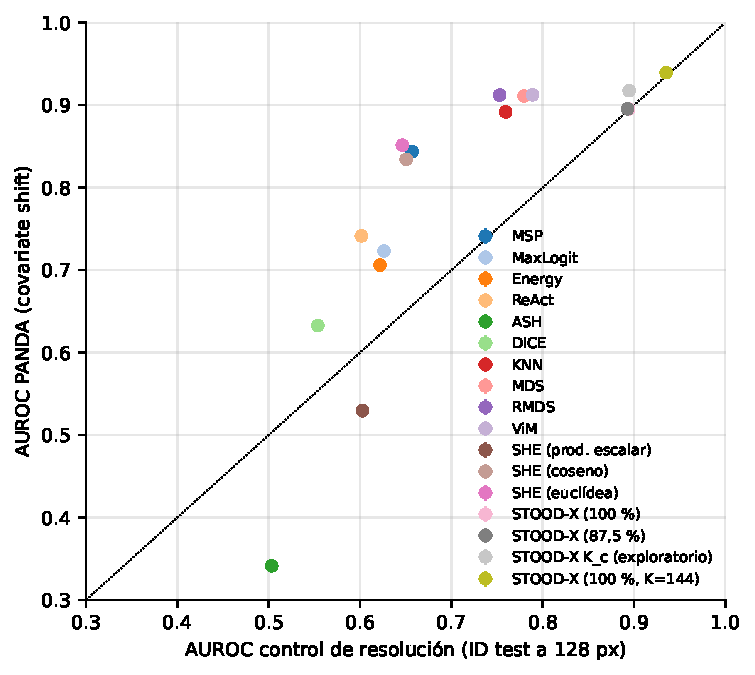
\includegraphics[width=0.7\textwidth]{img/cap10/fig4_panda_vs_control.pdf}
  \caption{AUROC en PANDA frente a AUROC en el control de resolución (test ID a 128\,px), un punto por método con sus IC. La diagonal indica la misma capacidad de detección en ambos conjuntos. Como PANDA difiere también en escala y en contenido de fondo, quedar por encima de la diagonal no permite atribuir la diferencia solo al cambio de centro. STOOD-X con $K = 500$ queda sobre la diagonal por la saturación de su estadístico.}
  \label{fig:ood-panda-control}
\end{figure}

\revisar{propuesta: matizar con las corrupciones sintéticas (\cref{sec:ood-corr-saturacion}): allí la saturación de \stoodx crece con la severidad (hasta el 86,4\,\% en pixelado 5) y el umbral del 95\,\% de \texttt{id\_val} ($-38{,}256$) queda por encima del valor saturado ($-38{,}691$), así que toda imagen saturada se rechaza; no se cambia el texto del autor}

\section{Corrupciones sintéticas: \emph{covariate shift} controlado}\label{sec:ood-corrupciones}

% Fuente: OpenOOD/results_corrupciones (metricas_celda.csv, exactitud_celda.csv, cec.csv,
% saturacion_stoodx.csv, correlacion_exactitud_auroc.csv) y su fase 8b (fase8b/*.csv). Metodología en la
% \cref{sec:corrupciones} (\cref{tab:corrupciones,fig:ejemplo-corrupciones}); CEC en la \cref{sec:cec}.
% Puntos de la introducción, en el orden en que se redactarían:
% - Diseño pareado: ID = las imágenes limpias del test; OOD = sus versiones corruptas en cada celda.
% - 9 corrupciones x niveles 1, 3 y 5 sobre las 12.618 imágenes del test ID (27 celdas, más la limpia).
% - Los mismos detectores y referencias (train limpio) que el resto del capítulo, sin reajuste.
% - En las tablas principales van 6 detectores: MSP, MDS, KNN, ViM, RMDS y STOOD-X 100 % (K = 500); el
%   resto (15 configuraciones en total), en el apéndice (\cref{sec:apc-corrupciones}) o donde se indique.
% - Dos preguntas distintas:
%   (1) ¿detecta el detector que la imagen está alterada? (\cref{sec:ood-corr-deteccion,sec:ood-corr-cec,sec:ood-corr-saturacion});
%   (2) ¿rechaza las imágenes alteradas que el clasificador clasifica mal? (\cref{sec:ood-corr-errores}).
\pendiente{introducción de la sección}

\subsection{Exactitud del clasificador ante las corrupciones}\label{sec:ood-corr-exactitud}

% Generado por scripts/generar_tablas.py a partir de results_corrupciones/exactitud_celda.csv. No editar a mano.
\begin{table}[tbp]
\centering
\scriptsize
\setlength{\tabcolsep}{3pt}
\caption{Exactitud del Swin-S (más alto es mejor) en cada corrupción y nivel de severidad, y caída respecto a la imagen limpia (exactitud 0{,}969 [0{,}966; 0{,}972]), con su IC debajo. IC del 95\,\% por \emph{bootstrap} pareado por imagen (1.000 réplicas, semilla 0).}
\label{tab:ood-corr-exactitud}
\begin{tabular}{lcccccc}
\toprule
& \multicolumn{3}{c}{Exactitud $\uparrow$} & \multicolumn{3}{c}{Caída respecto a la limpia} \\
\cmidrule(lr){2-4}\cmidrule(lr){5-7}
Corrupción & Nivel 1 & Nivel 3 & Nivel 5 & Nivel 1 & Nivel 3 & Nivel 5 \\
\midrule
Brillo & 0{,}965 & 0{,}910 & 0{,}796 & 0{,}004 & 0{,}059 & 0{,}173 \\
& {\tiny [0{,}961; 0{,}968]} & {\tiny [0{,}905; 0{,}915]} & {\tiny [0{,}789; 0{,}803]} & {\tiny [0{,}002; 0{,}006]} & {\tiny [0{,}054; 0{,}063]} & {\tiny [0{,}166; 0{,}180]} \\[2pt]
Saturación & 0{,}954 & 0{,}882 & 0{,}733 & 0{,}015 & 0{,}087 & 0{,}236 \\
& {\tiny [0{,}950; 0{,}957]} & {\tiny [0{,}876; 0{,}888]} & {\tiny [0{,}725; 0{,}741]} & {\tiny [0{,}012; 0{,}018]} & {\tiny [0{,}082; 0{,}093]} & {\tiny [0{,}228; 0{,}244]} \\[2pt]
Tono & 0{,}935 & 0{,}774 & 0{,}580 & 0{,}034 & 0{,}194 & 0{,}388 \\
& {\tiny [0{,}930; 0{,}939]} & {\tiny [0{,}768; 0{,}782]} & {\tiny [0{,}573; 0{,}589]} & {\tiny [0{,}030; 0{,}038]} & {\tiny [0{,}187; 0{,}201]} & {\tiny [0{,}379; 0{,}396]} \\[2pt]
Marcas & 0{,}966 & 0{,}959 & 0{,}929 & 0{,}003 & 0{,}010 & 0{,}040 \\
& {\tiny [0{,}963; 0{,}969]} & {\tiny [0{,}956; 0{,}962]} & {\tiny [0{,}925; 0{,}934]} & {\tiny [0{,}001; 0{,}004]} & {\tiny [0{,}007; 0{,}012]} & {\tiny [0{,}036; 0{,}044]} \\[2pt]
Burbujas & 0{,}967 & 0{,}894 & 0{,}811 & 0{,}002 & 0{,}074 & 0{,}158 \\
& {\tiny [0{,}964; 0{,}970]} & {\tiny [0{,}889; 0{,}900]} & {\tiny [0{,}804; 0{,}818]} & {\tiny [0{,}000; 0{,}003]} & {\tiny [0{,}069; 0{,}080]} & {\tiny [0{,}151; 0{,}165]} \\[2pt]
JPEG & 0{,}642 & 0{,}584 & 0{,}404 & 0{,}327 & 0{,}385 & 0{,}565 \\
& {\tiny [0{,}634; 0{,}650]} & {\tiny [0{,}575; 0{,}592]} & {\tiny [0{,}396; 0{,}412]} & {\tiny [0{,}318; 0{,}335]} & {\tiny [0{,}376; 0{,}394]} & {\tiny [0{,}556; 0{,}573]} \\[2pt]
Pixelado & 0{,}847 & 0{,}697 & 0{,}277 & 0{,}122 & 0{,}272 & 0{,}692 \\
& {\tiny [0{,}840; 0{,}853]} & {\tiny [0{,}689; 0{,}705]} & {\tiny [0{,}269; 0{,}285]} & {\tiny [0{,}116; 0{,}128]} & {\tiny [0{,}264; 0{,}280]} & {\tiny [0{,}683; 0{,}700]} \\[2pt]
Desenfoque & 0{,}637 & 0{,}380 & 0{,}287 & 0{,}332 & 0{,}588 & 0{,}681 \\
& {\tiny [0{,}629; 0{,}645]} & {\tiny [0{,}372; 0{,}389]} & {\tiny [0{,}280; 0{,}295]} & {\tiny [0{,}324; 0{,}340]} & {\tiny [0{,}579; 0{,}597]} & {\tiny [0{,}673; 0{,}689]} \\[2pt]
Movimiento & 0{,}910 & 0{,}642 & 0{,}433 & 0{,}059 & 0{,}327 & 0{,}536 \\
& {\tiny [0{,}905; 0{,}915]} & {\tiny [0{,}634; 0{,}650]} & {\tiny [0{,}425; 0{,}442]} & {\tiny [0{,}054; 0{,}063]} & {\tiny [0{,}319; 0{,}335]} & {\tiny [0{,}526; 0{,}545]} \\[2pt]
\bottomrule
\end{tabular}
\end{table}


\begin{figure}[tbp]
  \centering
  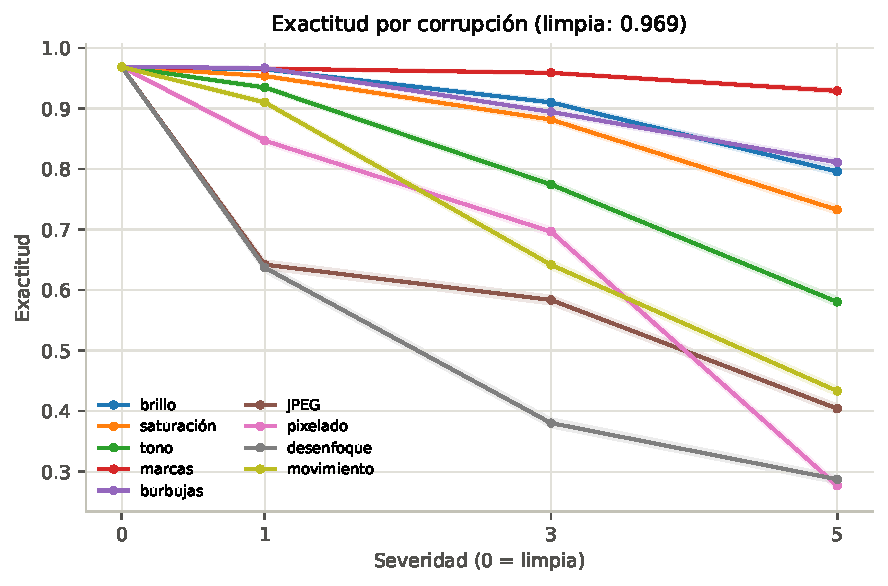
\includegraphics[width=0.75\textwidth]{img/cap10/corr_c_exactitud_severidad.pdf}
  \caption{Exactitud del Swin-S (más alto es mejor) frente al nivel de severidad (0 = imagen limpia; 1, 3 y 5), una línea por corrupción, con IC del 95\,\% por \emph{bootstrap}.}
  \label{fig:ood-corr-exactitud}
\end{figure}

% [propuesta de análisis] El brillo apenas afecta en el nivel 1: exactitud 0,965 [0,961; 0,968], caída
%   0,004 [0,002; 0,006]. Es coherente con que el brillo y el contraste formaban parte del aumento de datos
%   (\cref{sec:dataloader}), aunque eso no demuestra la causa.
% [propuesta de análisis] El modelo es frágil ante la compresión y el desenfoque ya en el nivel 1: JPEG 0,642
%   [0,634; 0,650] y desenfoque 0,637 [0,629; 0,645]. Con pixelado de nivel 5 cae a 0,277 [0,269; 0,285]
%   (la más baja de las 27 celdas; desenfoque 5: 0,287).
% [propuesta de análisis] Las marcas tienen un efecto pequeño (0,929 [0,925; 0,934] en el nivel 5; caída
%   0,040): son una sola mancha en una posición fija.
% [propuesta de análisis] Las calidades JPEG de Zhang (25, 15 y 7, \cref{tab:corrupciones}) son muy agresivas.
% Otras cifras: tono 5, 0,580; saturación 5, 0,733; burbujas 5, 0,811; movimiento 1, 0,910 y 5, 0,433.
\pendiente{análisis}
\pendiente{cita, si se quiere comparar con la compresión habitual de los escáneres}

\subsection{¿Detectan la alteración? AUROC y FPR@95}\label{sec:ood-corr-deteccion}

% Generado por scripts/generar_tablas.py a partir de results_corrupciones/metricas_celda.csv. No editar a mano.
\begin{table}
\centering
\scriptsize
\setlength{\tabcolsep}{3pt}
\caption{\AUROC (más alto es mejor) de los seis detectores principales en cada corrupción y nivel de severidad. ID: las imágenes limpias del test; OOD: sus versiones corruptas. En negrita, el mejor valor de cada fila. Las demás configuraciones y los IC del 95\,\% están en la \cref{tab:apc-corr-auroc}.}
\label{tab:ood-corr-auroc}
\begin{tabular*}{\linewidth}{@{\extracolsep{\fill}}llcccccc}
\toprule
Corrupción & Nivel & MSP & MDS & KNN & ViM & RMDS & STOOD-X (100\,\%) \\
\midrule
Brillo & 1 & 0{,}532 & 0{,}528 & 0{,}529 & 0{,}530 & 0{,}521 & \textbf{0{,}546} \\
 & 3 & 0{,}668 & 0{,}710 & 0{,}703 & 0{,}718 & 0{,}682 & \textbf{0{,}793} \\
 & 5 & 0{,}777 & 0{,}853 & 0{,}835 & 0{,}861 & 0{,}828 & \textbf{0{,}922} \\
\addlinespace[2pt]
Saturación & 1 & 0{,}574 & 0{,}606 & 0{,}592 & 0{,}610 & 0{,}574 & \textbf{0{,}658} \\
 & 3 & 0{,}693 & 0{,}775 & 0{,}756 & 0{,}782 & 0{,}742 & \textbf{0{,}853} \\
 & 5 & 0{,}794 & 0{,}873 & 0{,}851 & 0{,}879 & 0{,}853 & \textbf{0{,}932} \\
\addlinespace[2pt]
Tono & 1 & 0{,}576 & 0{,}595 & 0{,}594 & 0{,}601 & 0{,}598 & \textbf{0{,}675} \\
 & 3 & 0{,}713 & 0{,}777 & 0{,}781 & 0{,}782 & 0{,}793 & \textbf{0{,}865} \\
 & 5 & 0{,}756 & 0{,}831 & 0{,}832 & 0{,}837 & 0{,}850 & \textbf{0{,}925} \\
\addlinespace[2pt]
Marcas & 1 & 0{,}472 & 0{,}518 & 0{,}522 & 0{,}522 & 0{,}524 & \textbf{0{,}539} \\
 & 3 & 0{,}503 & 0{,}647 & 0{,}630 & 0{,}661 & 0{,}658 & \textbf{0{,}741} \\
 & 5 & 0{,}575 & 0{,}762 & 0{,}733 & 0{,}777 & 0{,}763 & \textbf{0{,}878} \\
\addlinespace[2pt]
Burbujas & 1 & 0{,}528 & 0{,}522 & 0{,}520 & 0{,}525 & 0{,}517 & \textbf{0{,}535} \\
 & 3 & 0{,}591 & 0{,}796 & 0{,}782 & 0{,}804 & 0{,}800 & \textbf{0{,}891} \\
 & 5 & 0{,}627 & 0{,}857 & 0{,}842 & 0{,}866 & 0{,}870 & \textbf{0{,}959} \\
\addlinespace[2pt]
JPEG & 1 & 0{,}690 & 0{,}781 & 0{,}782 & 0{,}787 & 0{,}798 & \textbf{0{,}897} \\
 & 3 & 0{,}740 & 0{,}826 & 0{,}824 & 0{,}830 & 0{,}850 & \textbf{0{,}936} \\
 & 5 & 0{,}827 & 0{,}909 & 0{,}899 & 0{,}913 & 0{,}911 & \textbf{0{,}983} \\
\addlinespace[2pt]
Pixelado & 1 & 0{,}636 & 0{,}755 & 0{,}743 & 0{,}767 & 0{,}737 & \textbf{0{,}868} \\
 & 3 & 0{,}729 & 0{,}846 & 0{,}829 & 0{,}856 & 0{,}841 & \textbf{0{,}951} \\
 & 5 & 0{,}974 & \textbf{0{,}993} & 0{,}986 & \textbf{0{,}993} & 0{,}977 & 0{,}992 \\
\addlinespace[2pt]
Desenfoque & 1 & 0{,}826 & 0{,}923 & 0{,}907 & 0{,}927 & 0{,}917 & \textbf{0{,}970} \\
 & 3 & 0{,}930 & 0{,}982 & 0{,}971 & 0{,}983 & 0{,}965 & \textbf{0{,}985} \\
 & 5 & 0{,}962 & \textbf{0{,}994} & 0{,}987 & \textbf{0{,}994} & 0{,}980 & 0{,}991 \\
\addlinespace[2pt]
Movimiento & 1 & 0{,}664 & 0{,}784 & 0{,}755 & 0{,}795 & 0{,}748 & \textbf{0{,}883} \\
 & 3 & 0{,}840 & 0{,}943 & 0{,}925 & 0{,}947 & 0{,}926 & \textbf{0{,}974} \\
 & 5 & 0{,}900 & 0{,}975 & 0{,}961 & 0{,}977 & 0{,}954 & \textbf{0{,}981} \\
\bottomrule
\end{tabular*}
\end{table}


\begin{figure}[tbp]
  \centering
  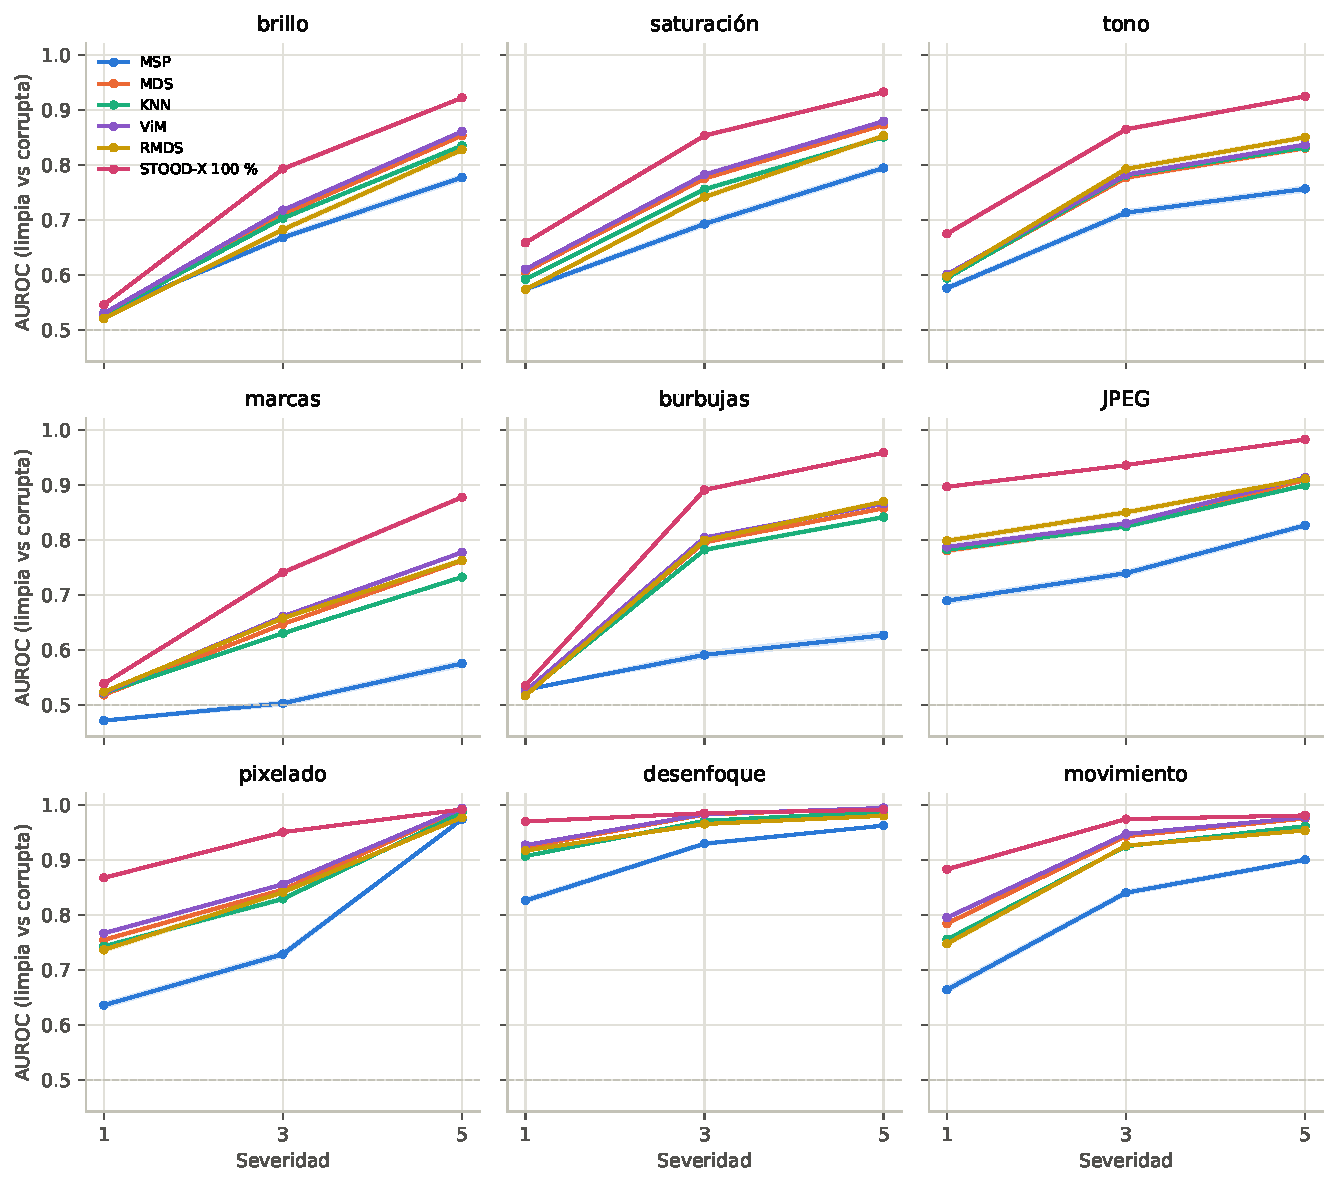
\includegraphics[width=\textwidth]{img/cap10/corr_b_auroc_severidad.pdf}
  \caption{\AUROC (más alto es mejor) frente al nivel de severidad de los seis detectores principales, un panel por corrupción, con bandas de IC del 95\,\% por \emph{bootstrap}. ID: las imágenes limpias; OOD: sus versiones corruptas.}
  \label{fig:ood-corr-auroc}
\end{figure}

% [propuesta de análisis] STOOD-X (100 %, K = 500) tiene el AUROC más alto en la mayoría de celdas, sobre
%   todo en los niveles bajos y medios. Ejemplos (comprobados): JPEG 1, 0,897 frente a 0,787 de ViM;
%   saturación 1, 0,658 frente a 0,610 (ViM); burbujas 3, 0,891 frente a 0,804 (ViM).
% Recuentos (metricas_celda.csv; entre los 6 detectores principales; los mismos entre las 14
%   configuraciones sin STOOD-X 87,5 %):
%   - AUROC: STOOD-X es el mejor en 25 de 27 celdas; en 24 su IC no se solapa con el del segundo (se
%     solapa en desenfoque 3, frente a ViM). No es el mejor en pixelado 5 (ViM 0,993 frente a 0,992) ni
%     en desenfoque 5 (ViM 0,994 frente a 0,991).
%   - FPR@95: STOOD-X es el mejor en 22 de 27; en 19 su IC no se solapa con el del segundo (se solapa en
%     saturación 3 y marcas 3, frente a ViM, y en tono 1, frente a MDS). No es el mejor en brillo 1
%     (ViM 0,927 frente a 0,928), saturación 1 (ViM 0,863 frente a 0,872), tono 3 (KNN 0,621 frente a
%     0,624), burbujas 1 (ViM 0,925 frente a 0,934) ni movimiento 1 (ViM 0,508 frente a 0,535).
% [propuesta de análisis] El orden del resto: ViM >= MDS > KNN ~ RMDS. Comprobado: ViM > MDS en AUROC en
%   27/27 celdas; MDS > KNN en 22/27; KNN > RMDS en 12/27. AUROC medio en las 27 celdas: STOOD-X 0,856,
%   ViM 0,797, MDS 0,791, RMDS 0,784, KNN 0,780, MSP 0,707.
% [propuesta de análisis] MSP es casi ciego en los niveles bajos: FPR@95 entre 0,899 (desenfoque 1) y
%   0,967 (pixelado 1) en el nivel 1; en marcas 1, AUROC 0,472.
% [propuesta de análisis] En brillo 1, todos los detectores dan un AUROC cercano a 0,5: entre 0,521 (RMDS) y
%   0,546 (STOOD-X) en los 6 principales; entre 0,497 (ReAct) y 0,546 en los 15. Coherente con el aumento de
%   datos (\cref{sec:dataloader}).
% [propuesta de análisis] Comparación con PANDA (\cref{sec:ood-panda}): aquí el cambio está aislado, así que
%   la sensibilidad de STOOD-X se puede atribuir a la corrupción. El artículo de STOOD-X no estudia este
%   aspecto, y es relevante en medicina.
% [propuesta de análisis] Matiz: con el criterio del espectro completo (\cref{def:deteccionfullspectrum})
%   estas imágenes se deberían aceptar. Aquí se adopta el criterio clínico, que la
%   \cref{sec:ood-corr-errores} pone a prueba imagen a imagen.
\pendiente{análisis}
\revisar{tono: comparación con lo que estudia el artículo de \stoodx}
\pendiente{análisis del autor: comparación con PANDA}

% Generado por scripts/generar_tablas.py a partir de results_corrupciones/metricas_celda.csv. No editar a mano.
\begin{table}[tbp]
\centering
\scriptsize
\setlength{\tabcolsep}{3pt}
\caption{\FPRn{95} (más bajo es mejor) de los seis detectores principales en cada corrupción y nivel de severidad. ID: las imágenes limpias del test; OOD: sus versiones corruptas. En negrita, el mejor valor de cada fila. Las demás configuraciones y los IC del 95\,\% están en la \cref{tab:apc-corr-fpr95}.}
\label{tab:ood-corr-fpr95}
\begin{tabular}{llcccccc}
\toprule
Corrupción & Nivel & MSP & MDS & KNN & ViM & RMDS & STOOD-X (100\,\%) \\
\midrule
Brillo & 1 & 0{,}946 & 0{,}930 & 0{,}933 & \textbf{0{,}927} & 0{,}948 & 0{,}928 \\
 & 3 & 0{,}942 & 0{,}746 & 0{,}808 & 0{,}732 & 0{,}926 & \textbf{0{,}702} \\
 & 5 & 0{,}947 & 0{,}507 & 0{,}601 & 0{,}482 & 0{,}741 & \textbf{0{,}401} \\
\addlinespace[2pt]
Saturación & 1 & 0{,}948 & 0{,}869 & 0{,}915 & \textbf{0{,}863} & 0{,}947 & 0{,}872 \\
 & 3 & 0{,}955 & 0{,}631 & 0{,}747 & 0{,}617 & 0{,}840 & \textbf{0{,}607} \\
 & 5 & 0{,}949 & 0{,}423 & 0{,}547 & 0{,}413 & 0{,}684 & \textbf{0{,}349} \\
\addlinespace[2pt]
Tono & 1 & 0{,}945 & 0{,}860 & 0{,}861 & 0{,}866 & 0{,}933 & \textbf{0{,}851} \\
 & 3 & 0{,}913 & 0{,}668 & \textbf{0{,}621} & 0{,}662 & 0{,}644 & 0{,}624 \\
 & 5 & 0{,}871 & 0{,}534 & 0{,}513 & 0{,}522 & 0{,}545 & \textbf{0{,}414} \\
\addlinespace[2pt]
Marcas & 1 & 0{,}964 & 0{,}937 & 0{,}938 & 0{,}937 & 0{,}948 & \textbf{0{,}928} \\
 & 3 & 0{,}967 & 0{,}811 & 0{,}840 & 0{,}784 & 0{,}927 & \textbf{0{,}763} \\
 & 5 & 0{,}961 & 0{,}600 & 0{,}673 & 0{,}559 & 0{,}815 & \textbf{0{,}532} \\
\addlinespace[2pt]
Burbujas & 1 & 0{,}949 & \textbf{0{,}925} & 0{,}931 & \textbf{0{,}925} & 0{,}947 & 0{,}934 \\
 & 3 & 0{,}982 & 0{,}591 & 0{,}595 & 0{,}571 & 0{,}618 & \textbf{0{,}521} \\
 & 5 & 0{,}986 & 0{,}443 & 0{,}446 & 0{,}421 & 0{,}348 & \textbf{0{,}167} \\
\addlinespace[2pt]
JPEG & 1 & 0{,}947 & 0{,}726 & 0{,}634 & 0{,}715 & 0{,}807 & \textbf{0{,}480} \\
 & 3 & 0{,}925 & 0{,}613 & 0{,}549 & 0{,}608 & 0{,}443 & \textbf{0{,}306} \\
 & 5 & 0{,}850 & 0{,}296 & 0{,}291 & 0{,}287 & 0{,}224 & \textbf{0{,}055} \\
\addlinespace[2pt]
Pixelado & 1 & 0{,}967 & 0{,}724 & 0{,}725 & 0{,}687 & 0{,}858 & \textbf{0{,}537} \\
 & 3 & 0{,}964 & 0{,}534 & 0{,}544 & 0{,}495 & 0{,}557 & \textbf{0{,}226} \\
 & 5 & 0{,}068 & 0{,}043 & 0{,}083 & 0{,}041 & 0{,}074 & \textbf{0{,}016} \\
\addlinespace[2pt]
Desenfoque & 1 & 0{,}899 & 0{,}305 & 0{,}310 & 0{,}295 & 0{,}224 & \textbf{0{,}158} \\
 & 3 & 0{,}245 & 0{,}103 & 0{,}142 & 0{,}098 & 0{,}116 & \textbf{0{,}047} \\
 & 5 & 0{,}084 & 0{,}034 & 0{,}072 & 0{,}033 & 0{,}072 & \textbf{0{,}019} \\
\addlinespace[2pt]
Movimiento & 1 & 0{,}942 & 0{,}536 & 0{,}602 & \textbf{0{,}508} & 0{,}818 & 0{,}535 \\
 & 3 & 0{,}918 & 0{,}225 & 0{,}253 & 0{,}209 & 0{,}200 & \textbf{0{,}108} \\
 & 5 & 0{,}724 & 0{,}127 & 0{,}162 & 0{,}116 & 0{,}132 & \textbf{0{,}040} \\
\bottomrule
\end{tabular}
\end{table}


% [propuesta de análisis] El mismo recuento con FPR@95: STOOD-X es el mejor en 22 de 27 celdas (19 con IC
%   sin solapar); cifras arriba.
\pendiente{análisis}
\revisar{tablas completas, con IC y el resto de detectores, en el apéndice C (\cref{sec:apc-corrupciones}): confirmar ubicación}

\subsection{¿Gradúan la severidad? CEC}\label{sec:ood-corr-cec}

% Generado por scripts/generar_tablas.py a partir de results_corrupciones/cec.csv. No editar a mano.
\begin{table}
\centering
\footnotesize
\setlength{\tabcolsep}{4pt}
\caption{CEC global (más bajo es mejor) de las 15 configuraciones de detectores, de menor a mayor, sobre las nueve corrupciones y los niveles 0, 1, 3 y 5. IC del 95\,\% por \emph{bootstrap} pareado por imagen (1.000 réplicas, semilla 0). Pares empatados: porcentaje de pares de niveles con la misma puntuación.}
\label{tab:ood-corr-cec}
\begin{tabular*}{\linewidth}{@{\extracolsep{\fill}}lccc}
\toprule
Detector & CEC $\downarrow$ & IC 95\,\% & Pares empatados (\%) \\
\midrule
ViM & 0{,}106 & [0{,}105; 0{,}108] & 0{,}000 \\
MDS & 0{,}109 & [0{,}107; 0{,}111] & 0{,}000 \\
KNN & 0{,}121 & [0{,}119; 0{,}123] & 0{,}000 \\
STOOD-X (100\,\%)$^{\ast}$ & 0{,}128 & -- & 7{,}30$^{\ast\ast}$ \\
STOOD-X (87,5\,\%)$^{\ast}$ & 0{,}128 & -- & 7{,}57$^{\ast\ast}$ \\
RMDS & 0{,}159 & [0{,}157; 0{,}162] & 0{,}000 \\
SHE (coseno) & 0{,}192 & [0{,}190; 0{,}195] & 0{,}000 \\
SHE (euclídea) & 0{,}196 & [0{,}193; 0{,}198] & 0{,}000 \\
SHE (prod.\ escalar) & 0{,}209 & [0{,}207; 0{,}211] & 0{,}000 \\
MSP & 0{,}284 & [0{,}281; 0{,}286] & 0{,}001 \\
MaxLogit & 0{,}311 & [0{,}309; 0{,}313] & 0{,}001 \\
Energy & 0{,}314 & [0{,}312; 0{,}316] & 0{,}000 \\
ReAct & 0{,}322 & [0{,}320; 0{,}325] & 0{,}001 \\
DICE & 0{,}408 & [0{,}404; 0{,}411] & 0{,}000 \\
ASH & 0{,}447 & [0{,}445; 0{,}450] & 0{,}010 \\
\bottomrule
\end{tabular*}

\smallskip
\parbox{\linewidth}{\scriptsize 0 = ordenación monótona; 0,5 = azar. La CEC de MSP es la métrica de Zhang et al.~\cite{zhang2022corruptions} adaptada a nuestros niveles. $^{\ast}$Los pares en los que los dos niveles tienen la puntuación saturada cuentan como empate; con empates exactos, la CEC es 0{,}138 [0{,}136; 0{,}139] (100\,\%) y 0{,}138 [0{,}136; 0{,}140] (87,5\,\%). $^{\ast\ast}$Pares con los dos niveles saturados.}
\end{table}


\begin{figure}[tbp]
  \centering
  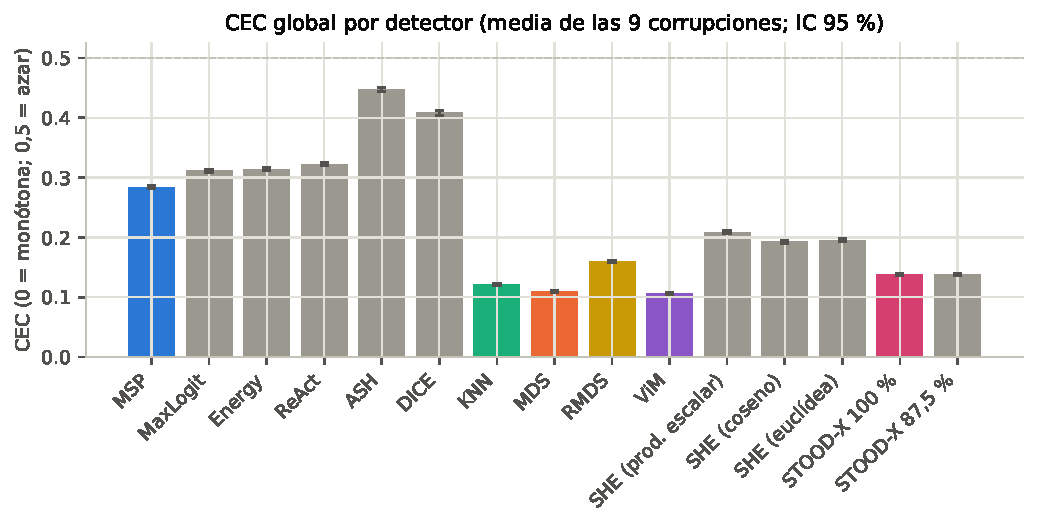
\includegraphics[width=0.8\textwidth]{img/cap10/corr_d_cec_barras.pdf}
  \caption{CEC global (más bajo es mejor; 0 = ordenación monótona, 0,5 = azar) de las 15 configuraciones de detectores, con IC del 95\,\% por \emph{bootstrap}. El detalle por corrupción está en la \cref{fig:apc-corr-cec-mapa}.}
  \label{fig:ood-corr-cec}
\end{figure}
\revisar{comprobar qué variante de la CEC de \stoodx muestra la figura (la de empates exactos, 0,138, o la de pares saturados como empate, 0,128): la tabla usa 0,128}

% [propuesta de análisis] Orden (cec.csv, fila global): ViM 0,106 < MDS 0,109 < KNN 0,121 < STOOD-X 0,128
%   (0,138 con empates exactos; 87,5 %: 0,128 y 0,138) < RMDS 0,159 < SHE 0,192-0,209 < MSP 0,284 <
%   MaxLogit 0,311, Energy 0,314 y ReAct 0,322 < DICE 0,408 < ASH 0,447.
%   Nota: la variante 0,128 está en cec.csv (columna CEC_saturadas_como_empate) sin IC; no se ha calculado.
% [propuesta de análisis] STOOD-X detecta mejor que ViM y MDS, pero ordena peor la severidad. El AUROC
%   compara poblaciones dentro de un nivel («¿hay cambio?»); la CEC sigue a cada imagen a lo largo de los
%   niveles («¿cuánto cambio hay?»).
% [propuesta de análisis] Mecanismo: el estadístico U de Mann-Whitney está acotado. Con separación completa
%   (U = n_1 n_2), la -z se satura (\cref{obs:u-empates}). Sin el término de empates de sigma:
%     z_máx = (n_1 n_2 / 2 - 1/2) / sqrt(n_1 n_2 (n_1 + n_2 + 1) / 12),
%   con la corrección de continuidad de scipy que usa stoodx_paper.py (z = (U - n_1 n_2/2 - 0,5)/sigma).
%   En stoodx_paper.py, n_1 = K = 500 y n_2 = K^2 = 250.000 (A: K distancias; B: K por cada uno de los K
%   vecinos; clases con n_c > K). Valor: z_máx = 38,6910841 (sin la corrección de continuidad,
%   38,6910844); saturacion_stoodx.csv da puntuaciones saturadas entre -38,6910841 y -38,6910841 (el término
%   de empates de sigma solo cambia el octavo decimal). ViM y MDS no tienen esa cota.
% [propuesta de análisis] Aun contando los pares saturados como empates, STOOD-X (0,128) queda por encima de
%   ViM (0,106): una prueba de rangos descarta la magnitud de las distancias.
% [propuesta de análisis] La relación CEC = (1 - tau_a)/2 se cumple con un error máximo de 1,1e-16
%   (comprobacion_cec_kendall.csv): enlaza con la proposición pendiente de la \cref{sec:cec}.
% Pares con los dos niveles saturados en STOOD-X: 7,30 % (100 %) y 7,57 % (87,5 %); por corrupción, de
%   0,68 % (marcas) a 27,25 % (desenfoque).
\pendiente{proposición del autor: valor de saturación de la $-z$ con separación completa}
\pendiente{análisis}
\revisar{tono: comparación de \stoodx con ViM y MDS}

\subsection{Saturación de STOOD-X}\label{sec:ood-corr-saturacion}

% Generado por scripts/generar_tablas.py a partir de results_corrupciones/saturacion_stoodx.csv. No editar a mano.
\begin{table}
\centering
\footnotesize
\setlength{\tabcolsep}{6pt}
\caption{Porcentaje de imágenes con la puntuación de \stoodx (100\,\%, $K=500$) saturada ($U=n_1n_2$; \cref{obs:u-empates}) en cada corrupción y nivel de severidad. Referencia: 0{,}62\,\% en las imágenes limpias del test.}
\label{tab:ood-corr-saturacion}
\begin{tabular*}{\linewidth}{@{\extracolsep{\fill}}lccc}
\toprule
Corrupción & Nivel 1 & Nivel 3 & Nivel 5 \\
\midrule
Brillo & 0{,}7 & 5{,}4 & 22{,}9 \\
Saturación & 2{,}3 & 13{,}0 & 28{,}4 \\
Tono & 2{,}7 & 20{,}9 & 33{,}6 \\
Marcas & 0{,}6 & 3{,}0 & 12{,}3 \\
Burbujas & 0{,}8 & 14{,}0 & 27{,}2 \\
JPEG & 25{,}8 & 31{,}1 & 45{,}9 \\
Pixelado & 14{,}9 & 32{,}6 & 86{,}4 \\
Desenfoque & 52{,}9 & 75{,}1 & 85{,}7 \\
Movimiento & 16{,}1 & 57{,}9 & 73{,}6 \\
\bottomrule
\end{tabular*}
\end{table}


% [propuesta de análisis] La saturación crece con la severidad: desenfoque 52,9/75,1/85,7 %, pixelado
%   14,9/32,6/86,4 %, movimiento 16,1/57,9/73,6 % y JPEG 25,8/31,1/45,9 % (comprobado). Imagen limpia:
%   0,62 %. La menor: marcas 1 (0,6 %) y brillo 1 (0,7 %).
% [propuesta de análisis] El umbral que acepta el 95 % de id_val (-38,256) está por encima del valor de
%   saturación (-38,691), así que todas las imágenes saturadas se rechazan (fase8b/decisiones.md;
%   umbral_fijo_celda.csv). En id_val satura el 0,61 % (100 %).
% [propuesta de análisis] Enlace con la \cref{sec:ood-panda}: en PANDA y en el control satura cerca de un
%   tercio con K = 500; aquí la saturación es graduable y crece con la severidad.
% La figura e_empates_saturacion (results_corrupciones/figuras_memoria) no se incluye: repite la tabla y el %
%   de pares empatados de la \cref{tab:ood-corr-cec}.
\pendiente{análisis}
\revisar{tono}

\subsection{¿Rechazan las imágenes alteradas que el clasificador clasifica mal?}\label{sec:ood-corr-errores}

% Fase 8b: imagen a imagen, la pregunta que la correlación por celdas solo trata de forma agregada. Positivo
% = imagen mal clasificada; puntuación de error = -s. AUROC_err con rangos medios (empates = 1/2).
% Correlación de Spearman por celdas (dato secundario; correlacion_exactitud_auroc.csv,
%   \cref{fig:apc-corr-dispersion}): rho entre la caída de exactitud y el AUROC sobre las 27 celdas: MSP 0,944,
%   MDS 0,908, KNN 0,933, ViM 0,906, RMDS 0,930, STOOD-X 0,931 (todas p < 1e-10); ASH 0,317 (p = 0,11) y DICE
%   0,270 (p = 0,17).
\pendiente{introducción de la subsección}

% Generado por scripts/generar_tablas.py a partir de results_corrupciones/results_corrupciones/fase8b/auroc_err_celda.csv y stoodx_variantes_auroc_err_celda.csv. No editar a mano.
\begin{table}[tbp]
\centering
\scriptsize
\setlength{\tabcolsep}{2.5pt}
\caption{\AUROC de detección de errores de clasificación (clase positiva: imagen mal clasificada; más alto es mejor) de los seis detectores principales, en la imagen limpia y en cada corrupción y nivel, con su IC debajo. Errores: número de imágenes mal clasificadas de las \num{12618} de la celda. En negrita, el mejor valor de cada fila. IC del 95\,\% por \emph{bootstrap} pareado por imagen (1.000 réplicas, semilla 0).}
\label{tab:ood-corr-auroc-err}
\begin{tabular}{llrcccccc}
\toprule
Corrupción & Nivel & Errores & MSP & MDS & KNN & ViM & RMDS & STOOD-X (100\,\%)$^{\ast}$ \\
\midrule
Limpia & -- & \num{395} & 0{,}855 & 0{,}939 & \textbf{0{,}950} & 0{,}939 & 0{,}923 & 0{,}846 \\
& & & {\tiny [0{,}826; 0{,}883]} & {\tiny [0{,}931; 0{,}947]} & {\tiny [0{,}943; 0{,}956]} & {\tiny [0{,}931; 0{,}947]} & {\tiny [0{,}906; 0{,}939]} & {\tiny [0{,}825; 0{,}866]} \\[1pt]
\midrule
Brillo & 1 & \num{445} & 0{,}856 & 0{,}936 & \textbf{0{,}948} & 0{,}935 & 0{,}919 & 0{,}818 \\
& & & {\tiny [0{,}830; 0{,}883]} & {\tiny [0{,}928; 0{,}944]} & {\tiny [0{,}941; 0{,}954]} & {\tiny [0{,}927; 0{,}943]} & {\tiny [0{,}901; 0{,}935]} & {\tiny [0{,}797; 0{,}839]} \\[1pt]
 & 3 & \num{1135} & 0{,}801 & 0{,}893 & \textbf{0{,}904} & 0{,}891 & 0{,}856 & 0{,}667 \\
& & & {\tiny [0{,}781; 0{,}819]} & {\tiny [0{,}884; 0{,}901]} & {\tiny [0{,}896; 0{,}911]} & {\tiny [0{,}882; 0{,}899]} & {\tiny [0{,}840; 0{,}870]} & {\tiny [0{,}649; 0{,}685]} \\[1pt]
 & 5 & \num{2577} & 0{,}754 & 0{,}827 & \textbf{0{,}837} & 0{,}826 & 0{,}803 & 0{,}594 \\
& & & {\tiny [0{,}741; 0{,}765]} & {\tiny [0{,}819; 0{,}834]} & {\tiny [0{,}829; 0{,}844]} & {\tiny [0{,}818; 0{,}833]} & {\tiny [0{,}793; 0{,}813]} & {\tiny [0{,}581; 0{,}607]} \\[1pt]
\addlinespace[2pt]
Saturación & 1 & \num{584} & 0{,}849 & 0{,}931 & \textbf{0{,}941} & 0{,}930 & 0{,}895 & 0{,}765 \\
& & & {\tiny [0{,}826; 0{,}872]} & {\tiny [0{,}923; 0{,}938]} & {\tiny [0{,}934; 0{,}947]} & {\tiny [0{,}923; 0{,}937]} & {\tiny [0{,}876; 0{,}912]} & {\tiny [0{,}742; 0{,}787]} \\[1pt]
 & 3 & \num{1493} & 0{,}805 & 0{,}883 & \textbf{0{,}895} & 0{,}882 & 0{,}859 & 0{,}658 \\
& & & {\tiny [0{,}790; 0{,}820]} & {\tiny [0{,}875; 0{,}890]} & {\tiny [0{,}888; 0{,}902]} & {\tiny [0{,}874; 0{,}889]} & {\tiny [0{,}848; 0{,}869]} & {\tiny [0{,}644; 0{,}674]} \\[1pt]
 & 5 & \num{3374} & 0{,}752 & 0{,}820 & \textbf{0{,}831} & 0{,}820 & 0{,}802 & 0{,}577 \\
& & & {\tiny [0{,}742; 0{,}762]} & {\tiny [0{,}812; 0{,}827]} & {\tiny [0{,}824; 0{,}839]} & {\tiny [0{,}812; 0{,}827]} & {\tiny [0{,}794; 0{,}810]} & {\tiny [0{,}565; 0{,}588]} \\[1pt]
\addlinespace[2pt]
Tono & 1 & \num{823} & 0{,}836 & 0{,}894 & \textbf{0{,}912} & 0{,}892 & 0{,}905 & 0{,}785 \\
& & & {\tiny [0{,}816; 0{,}855]} & {\tiny [0{,}884; 0{,}904]} & {\tiny [0{,}903; 0{,}920]} & {\tiny [0{,}882; 0{,}902]} & {\tiny [0{,}894; 0{,}916]} & {\tiny [0{,}770; 0{,}801]} \\[1pt]
 & 3 & \num{2847} & 0{,}766 & 0{,}823 & \textbf{0{,}834} & 0{,}820 & 0{,}829 & 0{,}700 \\
& & & {\tiny [0{,}755; 0{,}777]} & {\tiny [0{,}813; 0{,}832]} & {\tiny [0{,}825; 0{,}842]} & {\tiny [0{,}810; 0{,}829]} & {\tiny [0{,}819; 0{,}837]} & {\tiny [0{,}690; 0{,}710]} \\[1pt]
 & 5 & \num{5294} & 0{,}702 & \textbf{0{,}779} & 0{,}777 & 0{,}777 & 0{,}773 & 0{,}730 \\
& & & {\tiny [0{,}692; 0{,}711]} & {\tiny [0{,}770; 0{,}787]} & {\tiny [0{,}769; 0{,}785]} & {\tiny [0{,}769; 0{,}785]} & {\tiny [0{,}764; 0{,}781]} & {\tiny [0{,}722; 0{,}738]} \\[1pt]
\addlinespace[2pt]
Marcas & 1 & \num{430} & 0{,}818 & 0{,}934 & \textbf{0{,}946} & 0{,}934 & 0{,}919 & 0{,}833 \\
& & & {\tiny [0{,}787; 0{,}848]} & {\tiny [0{,}925; 0{,}943]} & {\tiny [0{,}939; 0{,}953]} & {\tiny [0{,}925; 0{,}942]} & {\tiny [0{,}901; 0{,}934]} & {\tiny [0{,}812; 0{,}854]} \\[1pt]
 & 3 & \num{518} & 0{,}834 & 0{,}914 & \textbf{0{,}932} & 0{,}913 & 0{,}922 & 0{,}741 \\
& & & {\tiny [0{,}807; 0{,}859]} & {\tiny [0{,}904; 0{,}923]} & {\tiny [0{,}924; 0{,}940]} & {\tiny [0{,}903; 0{,}922]} & {\tiny [0{,}908; 0{,}934]} & {\tiny [0{,}720; 0{,}763]} \\[1pt]
 & 5 & \num{895} & 0{,}831 & 0{,}887 & \textbf{0{,}907} & 0{,}886 & \textbf{0{,}907} & 0{,}700 \\
& & & {\tiny [0{,}814; 0{,}848]} & {\tiny [0{,}878; 0{,}895]} & {\tiny [0{,}899; 0{,}914]} & {\tiny [0{,}877; 0{,}894]} & {\tiny [0{,}898; 0{,}915]} & {\tiny [0{,}683; 0{,}717]} \\[1pt]
\addlinespace[2pt]
Burbujas & 1 & \num{417} & 0{,}826 & 0{,}934 & \textbf{0{,}947} & 0{,}933 & 0{,}924 & 0{,}825 \\
& & & {\tiny [0{,}796; 0{,}856]} & {\tiny [0{,}926; 0{,}942]} & {\tiny [0{,}939; 0{,}953]} & {\tiny [0{,}925; 0{,}941]} & {\tiny [0{,}906; 0{,}939]} & {\tiny [0{,}804; 0{,}847]} \\[1pt]
 & 3 & \num{1333} & 0{,}793 & 0{,}853 & \textbf{0{,}875} & 0{,}851 & 0{,}874 & 0{,}702 \\
& & & {\tiny [0{,}776; 0{,}810]} & {\tiny [0{,}844; 0{,}862]} & {\tiny [0{,}866; 0{,}883]} & {\tiny [0{,}842; 0{,}860]} & {\tiny [0{,}865; 0{,}883]} & {\tiny [0{,}690; 0{,}716]} \\[1pt]
 & 5 & \num{2385} & 0{,}727 & 0{,}799 & 0{,}812 & 0{,}796 & \textbf{0{,}818} & 0{,}687 \\
& & & {\tiny [0{,}713; 0{,}740]} & {\tiny [0{,}790; 0{,}808]} & {\tiny [0{,}804; 0{,}821]} & {\tiny [0{,}787; 0{,}806]} & {\tiny [0{,}809; 0{,}827]} & {\tiny [0{,}676; 0{,}698]} \\[1pt]
\addlinespace[2pt]
JPEG & 1 & \num{4516} & 0{,}694 & 0{,}782 & \textbf{0{,}796} & 0{,}779 & 0{,}792 & 0{,}676 \\
& & & {\tiny [0{,}684; 0{,}704]} & {\tiny [0{,}774; 0{,}790]} & {\tiny [0{,}788; 0{,}804]} & {\tiny [0{,}771; 0{,}787]} & {\tiny [0{,}785; 0{,}800]} & {\tiny [0{,}667; 0{,}686]} \\[1pt]
 & 3 & \num{5254} & 0{,}701 & 0{,}770 & \textbf{0{,}779} & 0{,}767 & 0{,}772 & 0{,}656 \\
& & & {\tiny [0{,}691; 0{,}711]} & {\tiny [0{,}762; 0{,}778]} & {\tiny [0{,}771; 0{,}787]} & {\tiny [0{,}759; 0{,}775]} & {\tiny [0{,}764; 0{,}780]} & {\tiny [0{,}647; 0{,}666]} \\[1pt]
 & 5 & \num{7519} & 0{,}623 & 0{,}714 & 0{,}707 & \textbf{0{,}715} & 0{,}703 & 0{,}599 \\
& & & {\tiny [0{,}614; 0{,}633]} & {\tiny [0{,}706; 0{,}724]} & {\tiny [0{,}697; 0{,}716]} & {\tiny [0{,}706; 0{,}725]} & {\tiny [0{,}694; 0{,}713]} & {\tiny [0{,}589; 0{,}608]} \\[1pt]
\addlinespace[2pt]
Pixelado & 1 & \num{1933} & 0{,}793 & 0{,}861 & \textbf{0{,}878} & 0{,}860 & 0{,}864 & 0{,}732 \\
& & & {\tiny [0{,}781; 0{,}805]} & {\tiny [0{,}853; 0{,}868]} & {\tiny [0{,}871; 0{,}885]} & {\tiny [0{,}853; 0{,}867]} & {\tiny [0{,}855; 0{,}872]} & {\tiny [0{,}720; 0{,}744]} \\[1pt]
 & 3 & \num{3828} & 0{,}758 & 0{,}817 & \textbf{0{,}830} & 0{,}816 & 0{,}823 & 0{,}661 \\
& & & {\tiny [0{,}749; 0{,}767]} & {\tiny [0{,}810; 0{,}824]} & {\tiny [0{,}823; 0{,}837]} & {\tiny [0{,}809; 0{,}824]} & {\tiny [0{,}816; 0{,}830]} & {\tiny [0{,}652; 0{,}671]} \\[1pt]
 & 5 & \num{9126} & 0{,}670 & 0{,}703 & \textbf{0{,}704} & \textbf{0{,}704} & 0{,}663 & 0{,}503 \\
& & & {\tiny [0{,}659; 0{,}680]} & {\tiny [0{,}693; 0{,}712]} & {\tiny [0{,}694; 0{,}714]} & {\tiny [0{,}695; 0{,}714]} & {\tiny [0{,}651; 0{,}674]} & {\tiny [0{,}496; 0{,}510]} \\[1pt]
\addlinespace[2pt]
Desenfoque & 1 & \num{4580} & 0{,}772 & 0{,}834 & \textbf{0{,}839} & 0{,}833 & 0{,}829 & 0{,}565 \\
& & & {\tiny [0{,}763; 0{,}781]} & {\tiny [0{,}827; 0{,}841]} & {\tiny [0{,}833; 0{,}846]} & {\tiny [0{,}826; 0{,}840]} & {\tiny [0{,}822; 0{,}836]} & {\tiny [0{,}555; 0{,}573]} \\[1pt]
 & 3 & \num{7819} & 0{,}722 & 0{,}750 & 0{,}749 & \textbf{0{,}752} & 0{,}726 & 0{,}474 \\
& & & {\tiny [0{,}714; 0{,}732]} & {\tiny [0{,}742; 0{,}760]} & {\tiny [0{,}740; 0{,}759]} & {\tiny [0{,}743; 0{,}761]} & {\tiny [0{,}716; 0{,}735]} & {\tiny [0{,}467; 0{,}482]} \\[1pt]
 & 5 & \num{8993} & 0{,}664 & 0{,}674 & 0{,}671 & \textbf{0{,}675} & 0{,}649 & 0{,}474 \\
& & & {\tiny [0{,}654; 0{,}674]} & {\tiny [0{,}664; 0{,}684]} & {\tiny [0{,}661; 0{,}682]} & {\tiny [0{,}665; 0{,}685]} & {\tiny [0{,}640; 0{,}660]} & {\tiny [0{,}468; 0{,}481]} \\[1pt]
\addlinespace[2pt]
Movimiento & 1 & \num{1134} & 0{,}834 & 0{,}903 & \textbf{0{,}914} & 0{,}903 & 0{,}895 & 0{,}665 \\
& & & {\tiny [0{,}818; 0{,}850]} & {\tiny [0{,}895; 0{,}909]} & {\tiny [0{,}907; 0{,}920]} & {\tiny [0{,}896; 0{,}909]} & {\tiny [0{,}885; 0{,}904]} & {\tiny [0{,}650; 0{,}681]} \\[1pt]
 & 3 & \num{4521} & 0{,}762 & 0{,}819 & \textbf{0{,}826} & 0{,}819 & 0{,}805 & 0{,}537 \\
& & & {\tiny [0{,}753; 0{,}772]} & {\tiny [0{,}812; 0{,}827]} & {\tiny [0{,}818; 0{,}833]} & {\tiny [0{,}811; 0{,}826]} & {\tiny [0{,}798; 0{,}814]} & {\tiny [0{,}528; 0{,}547]} \\[1pt]
 & 5 & \num{7152} & 0{,}712 & \textbf{0{,}764} & 0{,}755 & \textbf{0{,}764} & 0{,}743 & 0{,}532 \\
& & & {\tiny [0{,}702; 0{,}720]} & {\tiny [0{,}755; 0{,}772]} & {\tiny [0{,}746; 0{,}763]} & {\tiny [0{,}755; 0{,}772]} & {\tiny [0{,}734; 0{,}752]} & {\tiny [0{,}524; 0{,}539]} \\[1pt]
\bottomrule
\end{tabular}

\smallskip
\parbox{\linewidth}{\scriptsize $^{\ast}$Las imágenes con la puntuación saturada reciben la misma puntuación (empate real, que el AUROC cuenta como $\tfrac{1}{2}$); con la puntuación $-z$ original, su orden lo decide un término del orden de $10^{-8}$ (por ejemplo, pixelado 5: 0{,}503 con empates reales frente a 0{,}393 con la original; la variante original está en \texttt{stoodx\_variantes\_auroc\_err\_celda.csv}).}
\end{table}


\begin{figure}[tbp]
  \centering
  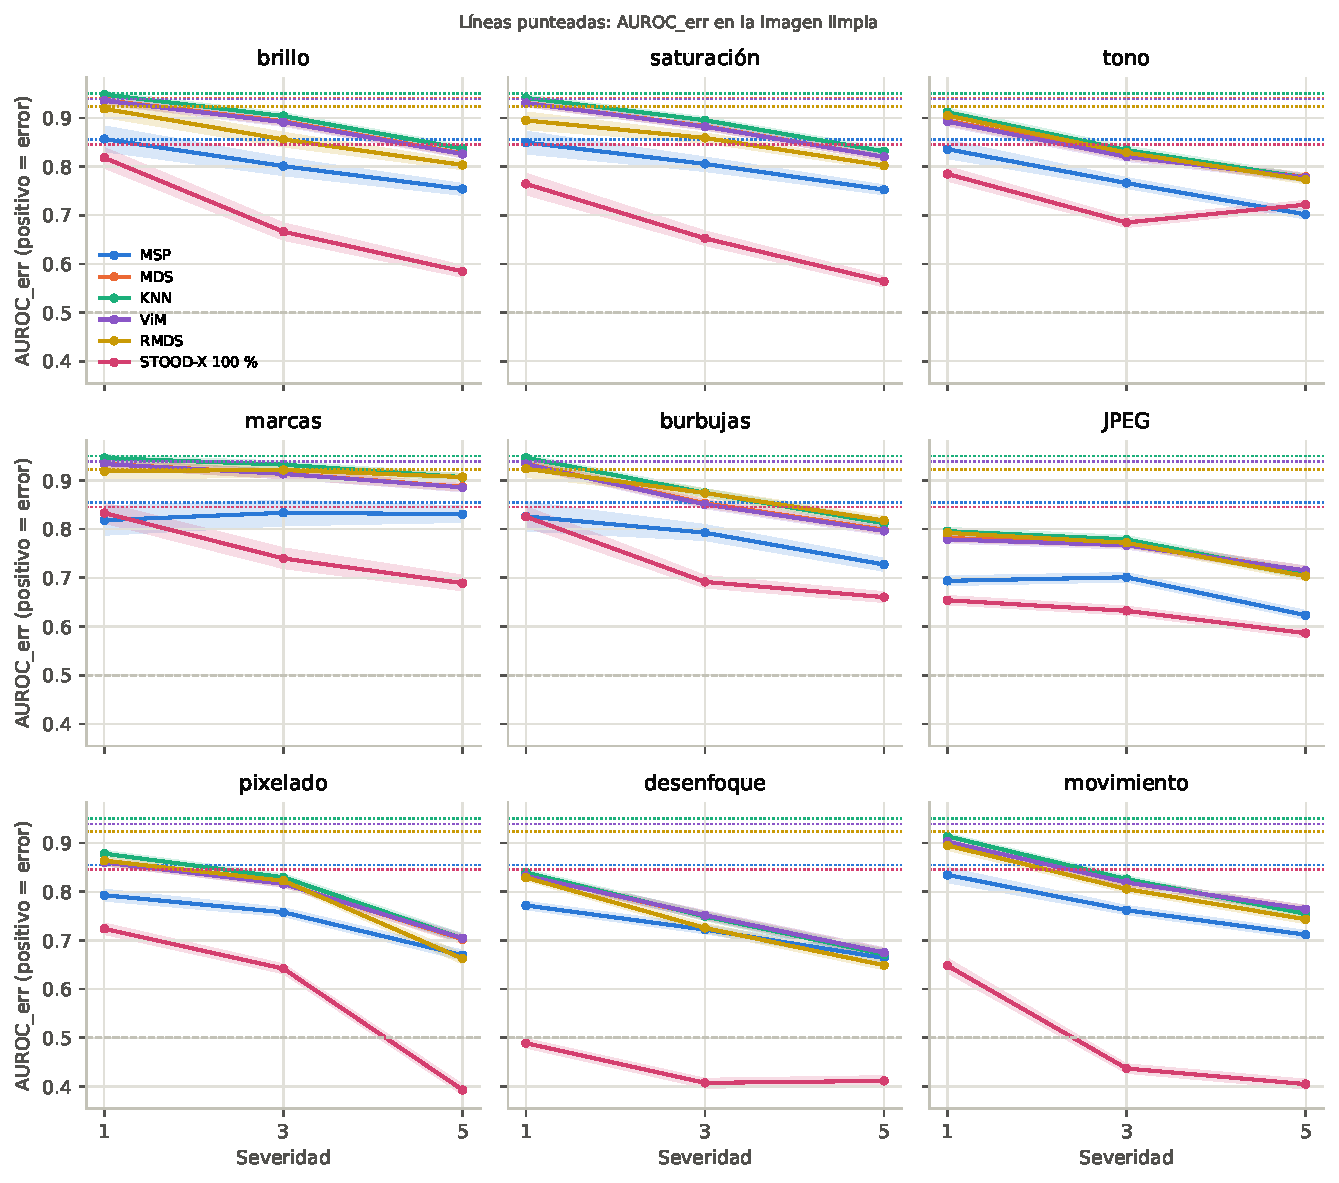
\includegraphics[width=\textwidth]{img/cap10/corr_fase8b_a_auroc_err_severidad.pdf}
  \caption{\AUROC de detección de errores de clasificación (clase positiva: imagen mal clasificada; más alto es mejor) frente al nivel de severidad de los seis detectores principales, un panel por corrupción, con bandas de IC del 95\,\% por \emph{bootstrap} y, en línea punteada, el valor en la imagen limpia. MDS y ViM se solapan casi por completo.}
  \label{fig:ood-corr-auroc-err}
\end{figure}
\revisar{la figura usa la puntuación original de \stoodx, no la variante con empates reales de la \cref{tab:ood-corr-auroc-err}; regenerarla con la variante principal}

% [propuesta de análisis] AUROC_err en la imagen limpia (comprobado): KNN 0,950, MDS 0,939, ViM 0,939,
%   RMDS 0,923, MSP 0,855 y STOOD-X 0,846 (STOOD-X - MSP = -0,010 [-0,039; 0,017], no concluyente). Los
%   detectores basados en características detectan los errores mejor que MSP incluso sin corrupción.
%   MSP es la referencia clásica para detectar errores de clasificación (Hendrycks y Gimpel, 2017; clave
%   hendrycks2017 en library.bib).
%   Hipótesis (no atribuir la causa sin evidencia): el label smoothing comprime la confianza
%   (\cref{sec:ood-familias}).
% [propuesta de análisis] AUROC_err en las corruptas: KNN, MDS y ViM obtienen valores de 0,671 a 0,948.
%   NO coincide «son los mejores en las 27 celdas»: los tres son los tres primeros en 17 de 27; en las
%   otras 10 RMDS entra entre los tres primeros (es el primero en marcas 5 y burbujas 5).
% [propuesta de análisis] STOOD-X queda por debajo de ViM y de MDS en las 27 celdas, con el IC de la
%   diferencia por debajo de 0 en todas (diferencias_auroc_err.csv). Con la puntuación original:
%   de -0,382 a -0,055 frente a ViM (de -0,382 a -0,057 frente a MDS); con empates reales, de -0,281 a
%   -0,047 frente a ViM (de -0,282 a -0,048 frente a MDS).
%   Frente a MSP (las dos variantes): peor con IC por debajo de 0 en 24 de 27; no concluyente en 2 (marcas 1,
%   burbujas 1) y mejor en 1 (tono 5: 0,020 [0,010; 0,030]). Por estimación puntual, por debajo en 25 de 27.
% [propuesta de análisis] Con la puntuación original, STOOD-X queda bajo 0,5 en pixelado 5 (0,393),
%   desenfoque 1 (0,489), 3 (0,407) y 5 (0,412) y movimiento 3 (0,437) y 5 (0,405). Con empates reales
%   se sitúa en torno a 0,5 (pixelado 5: 0,503; desenfoque 3 y 5: 0,474): no discrimina entre las
%   imágenes saturadas bien y mal clasificadas, porque en esas celdas la mayoría de unas y otras están
%   saturadas (pixelado 5: 86,7 % de los errores y 85,9 % de los aciertos; desenfoque 5: 84,2 % y 89,3 %;
%   desenfoque 3: 73,1 % y 78,2 %; movimiento 5: 76,3 % y 70,1 %).
\pendiente{análisis}
\revisar{tono}

% Generado por scripts/generar_tablas.py a partir de results_corrupciones/fase8b/umbral_fijo_celda.csv. No editar a mano.
\begin{table}[tbp]
\centering
\scriptsize
\setlength{\tabcolsep}{2.5pt}
\caption{Clasificación selectiva con un umbral fijo en una selección de celdas, para \stoodx (100\,\%), MSP y ViM (más alto es mejor en exactitud de las aceptadas, ganancia y captura). Exact.: exactitud de toda la celda; acept.: aceptación (fracción aceptada) y aceptadas; rech.: rechazadas. Umbral: percentil 5 de las puntuaciones de la validación ID (acepta el 95\,\% de \texttt{id\_val}); se acepta si la puntuación es mayor o igual. Ganancia (selectiva): exactitud de las aceptadas menos la de toda la celda. Captura (de errores): fracción de las imágenes mal clasificadas que se rechazan. Ganancia con su IC del 95\,\% por \emph{bootstrap} por imagen (1.000 réplicas). Todas las celdas, en la \cref{tab:apc-corr-umbral}.}
\label{tab:ood-corr-umbral}
\begin{tabular}{lllccccc}
\toprule
Celda & Exact.\ & Detector & Acept. & Exact.\ acept.\ $\uparrow$ & Exact.\ rech. & Ganancia $\uparrow$ & Captura $\uparrow$ \\
\midrule
Limpia & 0{,}969 & STOOD-X (100\,\%) & 0{,}951 & 0{,}980 & 0{,}743 & +0{,}012 {\tiny [+0{,}010; +0{,}014]} & 0{,}405 \\
 &  & MSP & 0{,}950 & 0{,}986 & 0{,}636 & +0{,}018 {\tiny [+0{,}016; +0{,}020]} & 0{,}585 \\
 &  & ViM & 0{,}951 & 0{,}984 & 0{,}679 & +0{,}015 {\tiny [+0{,}013; +0{,}017]} & 0{,}504 \\
\midrule
Brillo 5 & 0{,}796 & STOOD-X (100\,\%) & 0{,}317 & 0{,}854 & 0{,}769 & +0{,}059 {\tiny [+0{,}049; +0{,}068]} & 0{,}774 \\
 &  & MSP & 0{,}733 & 0{,}894 & 0{,}525 & +0{,}099 {\tiny [+0{,}093; +0{,}104]} & 0{,}621 \\
 &  & ViM & 0{,}615 & 0{,}931 & 0{,}579 & +0{,}135 {\tiny [+0{,}129; +0{,}142]} & 0{,}793 \\
\midrule
JPEG 5 & 0{,}404 & STOOD-X (100\,\%) & 0{,}061 & 0{,}661 & 0{,}387 & +0{,}257 {\tiny [+0{,}225; +0{,}289]} & 0{,}965 \\
 &  & MSP & 0{,}644 & 0{,}467 & 0{,}290 & +0{,}063 {\tiny [+0{,}057; +0{,}069]} & 0{,}424 \\
 &  & ViM & 0{,}503 & 0{,}533 & 0{,}273 & +0{,}129 {\tiny [+0{,}121; +0{,}137]} & 0{,}605 \\
\midrule
Pixelado 5 & 0{,}277 & STOOD-X (100\,\%) & 0{,}013 & 0{,}213 & 0{,}278 & $-$0{,}063 {\tiny [$-$0{,}123; $-$0{,}001]} & 0{,}986 \\
 &  & MSP & 0{,}140 & 0{,}506 & 0{,}240 & +0{,}229 {\tiny [+0{,}208; +0{,}251]} & 0{,}905 \\
 &  & ViM & 0{,}038 & 0{,}593 & 0{,}264 & +0{,}316 {\tiny [+0{,}272; +0{,}358]} & 0{,}979 \\
\midrule
Desenfoque 3 & 0{,}380 & STOOD-X (100\,\%) & 0{,}049 & 0{,}287 & 0{,}385 & $-$0{,}094 {\tiny [$-$0{,}129; $-$0{,}060]} & 0{,}944 \\
 &  & MSP & 0{,}295 & 0{,}664 & 0{,}262 & +0{,}283 {\tiny [+0{,}271; +0{,}298]} & 0{,}840 \\
 &  & ViM & 0{,}102 & 0{,}930 & 0{,}318 & +0{,}549 {\tiny [+0{,}533; +0{,}564]} & 0{,}988 \\
\midrule
Movimiento 5 & 0{,}433 & STOOD-X (100\,\%) & 0{,}043 & 0{,}356 & 0{,}437 & $-$0{,}077 {\tiny [$-$0{,}118; $-$0{,}040]} & 0{,}951 \\
 &  & MSP & 0{,}387 & 0{,}661 & 0{,}289 & +0{,}228 {\tiny [+0{,}217; +0{,}238]} & 0{,}769 \\
 &  & ViM & 0{,}163 & 0{,}878 & 0{,}347 & +0{,}445 {\tiny [+0{,}429; +0{,}459]} & 0{,}965 \\
\bottomrule
\end{tabular}
\end{table}


% Celdas elegidas: limpia, brillo 5, JPEG 5, pixelado 5, desenfoque 3 y movimiento 5 (las tres últimas, con
% ganancia selectiva negativa de STOOD-X; desenfoque 5 también la tiene: -0,055). Todas, en la
% \cref{tab:apc-corr-umbral}.
% [propuesta de análisis] Con el umbral del 95 % de id_val, STOOD-X rechaza casi todo en las severidades
%   altas: acepta el 4,9 % en desenfoque 3 y el 4,3 % en movimiento 5 (pixelado 5: 1,3 %; desenfoque 5:
%   1,8 %; JPEG 5: 6,1 %).
% [propuesta de análisis] Su ganancia selectiva llega a ser negativa (comprobado): pixelado 5, -0,063;
%   desenfoque 3, -0,094; desenfoque 5, -0,055; movimiento 5, -0,077. Las pocas imágenes que acepta no
%   están mejor clasificadas que la media.
% [propuesta de análisis] ViM, en cambio, acepta más y lo que acepta está mucho mejor clasificado:
%   desenfoque 3, aceptación 0,102 con exactitud de las aceptadas 0,930 frente a 0,380 de la celda.
% Captura de errores en esas celdas: STOOD-X 0,944-0,986; ViM 0,965-0,988 (desenfoque 3: 0,988).
\pendiente{análisis}
\revisar{tono}

% Generado por scripts/generar_tablas.py a partir de results_corrupciones/fase8b/aurc.csv. No editar a mano.
\begin{table}[tbp]
\centering
\footnotesize
\setlength{\tabcolsep}{4pt}
\caption{Área bajo la curva riesgo-cobertura (AURC; más bajo es mejor) conjunta de las imágenes limpias y las 27 celdas (\num{353304} imágenes; tasa de error global 0{,}258), al aceptar las imágenes de mayor a menor puntuación. Oráculo: rechaza primero los errores; azar: riesgo constante. IC del 95\,\% por \emph{bootstrap} por imagen original (cada réplica arrastra sus 28 versiones).}
\label{tab:ood-corr-aurc}
\begin{tabular}{lcc}
\toprule
Detector & AURC $\downarrow$ & IC 95\,\% \\
\midrule
Oráculo & 0{,}037 & [0{,}036; 0{,}038] \\
\midrule
KNN & 0{,}072 & [0{,}070; 0{,}074] \\
MDS & 0{,}074 & [0{,}072; 0{,}075] \\
ViM & 0{,}074 & [0{,}072; 0{,}076] \\
RMDS & 0{,}079 & [0{,}077; 0{,}081] \\
STOOD-X (100\,\%)$^{\ast}$ & 0{,}108 & [0{,}106; 0{,}111] \\
MSP & 0{,}124 & [0{,}121; 0{,}127] \\
\midrule
Azar & 0{,}258 & [0{,}255; 0{,}262] \\
\bottomrule
\end{tabular}

\smallskip
\parbox{\linewidth}{\scriptsize $^{\ast}$Imágenes saturadas con la misma puntuación (empate real); con la puntuación original, 0{,}113 [0{,}110; 0{,}115].}
\end{table}


\begin{figure}[tbp]
  \centering
  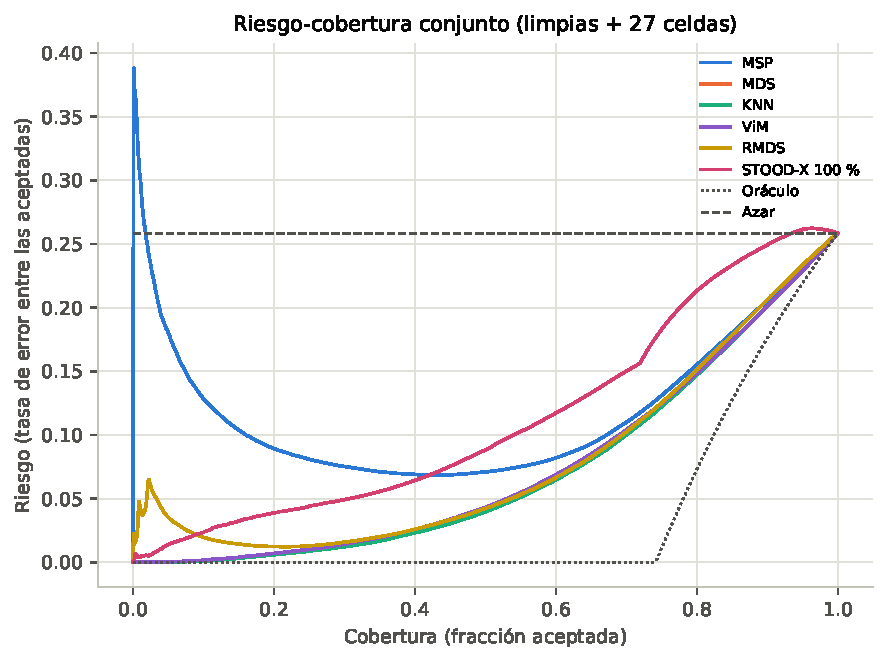
\includegraphics[width=0.75\textwidth]{img/cap10/corr_fase8b_c_riesgo_cobertura.pdf}
  \caption{Curvas riesgo-cobertura conjuntas (imágenes limpias y las 27 celdas) de los seis detectores principales, con el oráculo y el azar. Riesgo: tasa de error entre las imágenes aceptadas (más bajo es mejor). La curva de MDS queda tapada por la de ViM.}
  \label{fig:ood-corr-riesgo-cobertura}
\end{figure}
\revisar{la figura usa la puntuación original de \stoodx (AURC 0,113), no la variante con empates reales (0,108) de la \cref{tab:ood-corr-aurc}}

% [propuesta de análisis] AURC conjunto (comprobado; oráculo 0,037; azar 0,258): KNN 0,072 ~ MDS 0,074 ~
%   ViM 0,074 < RMDS 0,079 < STOOD-X 0,108 (0,113 con la puntuación original) < MSP 0,124.
% [propuesta de análisis] Lectura propuesta: son dos tareas distintas y complementarias.
%   - STOOD-X es el mejor para avisar de que la imagen está alterada: un control de calidad a nivel de
%     imagen que rechaza en bloque la adquisición defectuosa.
%   - KNN, MDS y ViM son los mejores para decidir en qué imágenes alteradas se puede confiar:
%     clasificación selectiva.
%   - Esto cumple el criterio clínico en las dos vías: STOOD-X rechaza casi todo lo muy corrupto, donde la
%     exactitud es baja (0,380 en desenfoque 3), aunque no distinga dentro de ello.
% Cautelas:
%   - Algunas celdas tienen pocos errores (395 en la limpia; 417-445 en burbujas 1, marcas 1 y brillo 1):
%     sus IC son más anchos.
%   - El AURC conjunto mezcla severidades.
%   - El umbral sale de id_val (puntuaciones en GPU) y se aplica a puntuaciones calculadas en CPU: en el
%     test limpio, Spearman >= 0,9999998. Con un umbral fijado en el test limpio, las diferencias son
%     <= 0,010 en MSP, STOOD-X y ViM, pero llegan a 0,012 (aceptación), 0,013 (exactitud de las aceptadas)
%     y 0,020 (captura de errores) en RMDS (fase8b/resumen.md).
%   - El bootstrap es por imagen.
\pendiente{análisis del autor}
\revisar{tono}


\section{Far-OOD}\label{sec:ood-far}

Finalmente, en Textures, STOOD-X obtiene el mejor resultado (AUROC 0,991 con $K = 500$ y 0,993 con $K = 144$), lo que confirma, como era de esperar, que las imágenes ajenas al contexto médico se detectan sin dificultad. 
Esta mayor dificultad de detecciónd de Near-OOD frente a Far-OOD coincide con los resultados también obtenidos en ~\cite{openood15}.
No obstante, con MDS (0,956) Textures resulta más difícil de detectar que TUM, NORM o LYM, lo que indica que la dificultad que encuentra cada detector no coincide necesariamente con la distancia semántica intuitiva.
% Generado por scripts/generar_tablas.py a partir de results_ood/faseC_K144/tabla_principal.csv. No editar a mano.
\begin{table}
\centering
\footnotesize
\setlength{\tabcolsep}{4pt}
\caption{Far-OOD (DTD): \AUROC y \CCRn{5} (más alto es mejor) y \FPRn{95} (más bajo es mejor) de los 17 métodos. IC del 95\,\% por \emph{bootstrap} (1.000 remuestreos estratificados, semilla 0). Clase positiva: OOD. En negrita, el mejor valor entre los métodos no exploratorios. $^{a}$ASH reduce la exactitud ID al 68{,}3\,\%. $^{\dagger}$Variante exploratoria ($K_c=\min(500,\lfloor n_c/2\rfloor)$), propuesta tras ver datos OOD; no es el método principal. $^{\ddagger}$100\,\% de las características y $K=144$, elegido solo con la validación ID (\cref{sec:stoodx-seleccion-k}); el resto de filas de \stoodx usan $K=500$, el valor del artículo.}
\label{tab:ood-far}
\begin{tabular}{lccc}
\toprule
Método & \AUROC $\uparrow$ [IC 95\,\%] & \FPRn{95} $\downarrow$ [IC 95\,\%] & \CCRn{5} $\uparrow$ \\
\midrule
\multicolumn{4}{@{}l}{\textit{Basados en logits}} \\
MSP & 0{,}876 [0{,}870; 0{,}882] & 0{,}780 [0{,}727; 0{,}830] & 0{,}217 \\
MaxLogit & 0{,}824 [0{,}817; 0{,}831] & 0{,}839 [0{,}805; 0{,}867] & 0{,}158 \\
Energy & 0{,}818 [0{,}811; 0{,}825] & 0{,}843 [0{,}805; 0{,}878] & 0{,}154 \\
\midrule
\multicolumn{4}{@{}l}{\textit{Modificación de activaciones}} \\
ReAct & 0{,}820 [0{,}813; 0{,}827] & 0{,}837 [0{,}816; 0{,}859] & 0{,}160 \\
ASH$^{a}$ & 0{,}549 [0{,}539; 0{,}559] & 0{,}993 [0{,}990; 0{,}994] & 0{,}004 \\
DICE & 0{,}436 [0{,}427; 0{,}444] & 0{,}999 [0{,}998; 1{,}000] & 0{,}001 \\
\midrule
\multicolumn{4}{@{}l}{\textit{Características y distancias}} \\
KNN & 0{,}936 [0{,}933; 0{,}939] & 0{,}214 [0{,}204; 0{,}225] & 0{,}785 \\
MDS & 0{,}956 [0{,}953; 0{,}958] & 0{,}181 [0{,}169; 0{,}190] & 0{,}816 \\
RMDS & 0{,}942 [0{,}939; 0{,}945] & 0{,}156 [0{,}148; 0{,}164] & 0{,}840 \\
ViM & 0{,}959 [0{,}956; 0{,}961] & 0{,}170 [0{,}160; 0{,}179] & 0{,}827 \\
SHE (prod.\ escalar) & 0{,}802 [0{,}796; 0{,}809] & 0{,}646 [0{,}637; 0{,}655] & 0{,}353 \\
SHE (coseno) & 0{,}898 [0{,}894; 0{,}902] & 0{,}387 [0{,}369; 0{,}407] & 0{,}611 \\
SHE (euclídea) & 0{,}899 [0{,}895; 0{,}903] & 0{,}422 [0{,}397; 0{,}443] & 0{,}576 \\
\midrule
\multicolumn{4}{@{}l}{\textit{STOOD-X}} \\
STOOD-X (100\,\%) & 0{,}991 [0{,}989; 0{,}992] & 0{,}028 [0{,}024; 0{,}033] & 0{,}949 \\
STOOD-X ($K=144$)$^{\ddagger}$ & \textbf{0{,}993} [0{,}992; 0{,}994] & \textbf{0{,}020} [0{,}018; 0{,}023] & \textbf{0{,}955} \\
STOOD-X (87,5\,\%) & 0{,}990 [0{,}989; 0{,}992] & 0{,}030 [0{,}025; 0{,}034] & 0{,}948 \\
STOOD-X $K_c$$^{\dagger}$ & 0{,}989 [0{,}988; 0{,}990] & 0{,}033 [0{,}028; 0{,}038] & 0{,}946 \\
\bottomrule
\end{tabular}
\end{table}

\revisar{añadido el AUROC con $K = 144$; quitado el punto suelto tras la tabla}


\section{Métodos basados en logits y en modificación de activaciones}\label{sec:ood-familias}

\textbf{Métodos basados en logits y en modificación de activaciones.} MSP supera a MaxLogit y a Energy en los nueve conjuntos, al contrario de lo habitual en la literatura. Una explicación plausible es el uso de \emph{label smoothing} durante el entrenamiento, que comprime la escala de los logits; comprobarlo requeriría entrenar el modelo sin esta técnica. Los métodos que modifican activaciones, diseñados para redes con activaciones ReLU y BatchNorm, no se trasladan bien a un Swin Transformer con LayerNorm. ReAct mejora a Energy, pero no a MSP. DICE queda por debajo de Energy en ocho de los nueve conjuntos, con un AUROC inferior al azar en DTD (0,436). ASH colapsa por completo: al redistribuir la suma de las activaciones, que es negativa en el 27,5\,\% de las imágenes, invierte los logits y reduce la exactitud ID al 68,3\,\%. Por último, SHE con producto escalar resulta irregular (0,795), mientras que sus variantes con distancia coseno (0,938) y euclídea (0,942) mejoran notablemente, lo que apunta de nuevo a la incompatibilidad entre las características con signo del Swin y los supuestos del método.
\revisar{«al contrario de lo habitual en la literatura»: falta cita}
\revisar{ReAct mejora a Energy en ocho de los nueve conjuntos; en el control de resolución queda por debajo (0,602 frente a 0,622)}
\revisar{el 27,5\,\% se midió en la validación ID}

% Generado por scripts/generar_tablas.py a partir de results_ood/faseC_K144/tabla_principal.csv. No editar a mano.
\begin{table}
\centering
\scriptsize
\setlength{\tabcolsep}{2.5pt}
\caption{Métodos basados en logits, en la modificación de activaciones y variantes de SHE: \AUROC (más alto es mejor) en los nueve conjuntos y exactitud ID de la clasificación resultante. Clase positiva: OOD. $^{a}$ASH modifica las características y con ellas la predicción.}
\label{tab:ood-familias}
\begin{tabular*}{\linewidth}{@{\extracolsep{\fill}}lcccccccccc}
\toprule
Método & TUM+NORM & TUM & NORM & STR & LYM & MUS & PANDA & Control 128\,px & DTD & Exact.\ ID (\%) \\
\midrule
\multicolumn{11}{@{}l}{\textit{Basados en logits}} \\
MSP & 0{,}876 & 0{,}873 & 0{,}880 & 0{,}823 & 0{,}854 & 0{,}740 & 0{,}843 & 0{,}657 & 0{,}876 & 96{,}87 \\
MaxLogit & 0{,}828 & 0{,}815 & 0{,}848 & 0{,}767 & 0{,}741 & 0{,}607 & 0{,}723 & 0{,}626 & 0{,}824 & 96{,}87 \\
Energy & 0{,}821 & 0{,}807 & 0{,}844 & 0{,}759 & 0{,}727 & 0{,}589 & 0{,}706 & 0{,}622 & 0{,}818 & 96{,}87 \\
\midrule
\multicolumn{11}{@{}l}{\textit{Modificación de activaciones}} \\
ReAct & 0{,}861 & 0{,}856 & 0{,}868 & 0{,}798 & 0{,}835 & 0{,}643 & 0{,}741 & 0{,}602 & 0{,}820 & 96{,}89 \\
ASH$^{a}$ & 0{,}546 & 0{,}496 & 0{,}628 & 0{,}544 & 0{,}504 & 0{,}361 & 0{,}341 & 0{,}503 & 0{,}549 & 68{,}33 \\
DICE & 0{,}592 & 0{,}581 & 0{,}609 & 0{,}581 & 0{,}831 & 0{,}525 & 0{,}633 & 0{,}554 & 0{,}436 & 96{,}84 \\
\midrule
\multicolumn{11}{@{}l}{\textit{Características y distancias}} \\
SHE (prod.\ escalar) & 0{,}795 & 0{,}746 & 0{,}875 & 0{,}780 & 0{,}647 & 0{,}660 & 0{,}530 & 0{,}603 & 0{,}802 & 96{,}87 \\
SHE (coseno) & 0{,}938 & 0{,}931 & 0{,}948 & 0{,}898 & 0{,}914 & 0{,}837 & 0{,}834 & 0{,}651 & 0{,}898 & 96{,}87 \\
SHE (euclídea) & 0{,}942 & 0{,}937 & 0{,}950 & 0{,}902 & 0{,}928 & 0{,}845 & 0{,}851 & 0{,}646 & 0{,}899 & 96{,}87 \\
\bottomrule
\end{tabular*}
\end{table}


% Las cifras de SHE (0,795; 0,938; 0,942) son del near-OOD principal (TUM+NORM).

\section{Hipótesis gaussiana de MDS}\label{sec:ood-mds-gaussiana}

% Fuente: scripts/figura_qq_mahalanobis.py sobre OpenOOD/features/completo (Swin-S, D = 768).
% mu_c y Sigma estimadas con id_train (90.800 imágenes), como en el postprocesador MDS de OpenOOD;
% -min_c d^2 reproduce las puntuaciones MDS de results_ood/faseA_2026-10-20_11-19-35/scores_mds.npz.
% Medianas de d^2 en el test ID (mediana de chi^2_768: 767,3): Adenocarcinoma_ductal 175,5;
% Carcinoma_intraductal 3604,8; Estroma 343,8; Glandulas_no_neoplasicas 240,5; Gleason_3 2787,3;
% Gleason_4_cribiformes 484,0; Gleason_4_fusionadas 951,4; Gleason_4_glomeruloide 9074,7;
% Gleason_4_pobremente_formadas 5261,1; Gleason_5_comedonecrosis 3227,1; Gleason_5_no_glandulas 578,4;
% Inflamatorio 1805,4; No_Cancer 2114,4; PIN_de_alto_grado 395,2.

MDS supone que, condicionadas a la clase, las características de la penúltima capa siguen gaussianas con una covarianza común (\cref{def:mds}). Es uno de los detectores más consistentes del estudio, con un \AUROC medio de 0,926 (\cref{tab:ood-global}), por lo que cabe preguntarse si las clases siguen realmente esa distribución.

Para comprobarlo se estiman las medias $\mu_c$ y la covarianza común $\Sigma$ con las \num{90800} imágenes de entrenamiento, igual que en MDS, y se calcula la distancia de Mahalanobis $d^2$ de cada una de las \num{12618} imágenes del test ID a su clase verdadera. Si la hipótesis se cumple, $d^2$ sigue una $\chi^2_{768}$ (\cref{prop:mahalanobis-chi2}), de modo que el Q-Q plot de las distancias de cada clase frente a la $\chi^2_{768}$ (\cref{sec:qq-plot}) debería quedar sobre la recta $y = x$. El experimento se ha implementado en Python con NumPy, scikit-learn (\texttt{EmpiricalCovariance}, el mismo estimador de la covarianza que usa el postprocesador MDS de OpenOOD), SciPy (cuantiles de la $\chi^2$) y Matplotlib, sobre las características del Swin-S ya exportadas. Se ha comprobado que, con estas estimaciones, la distancia mínima a las clases reproduce las puntuaciones de MDS del test ID usadas en este capítulo.

También se podría haber aplicado el test de Lilliefors~\cite{lilliefors1967} a las primeras componentes principales. Cualquier proyección lineal de una gaussiana es gaussiana, así que bastaría con que una sola componente no fuese normal para rechazar la hipótesis: se aplicaría el test a la primera componente y, si no se rechazara, a la segunda y a la tercera. No ha hecho falta, porque el Q-Q plot ya muestra que la hipótesis no se cumple (\cref{fig:ood-qq-mahalanobis}).

\begin{figure}[tbp]
  \centering
  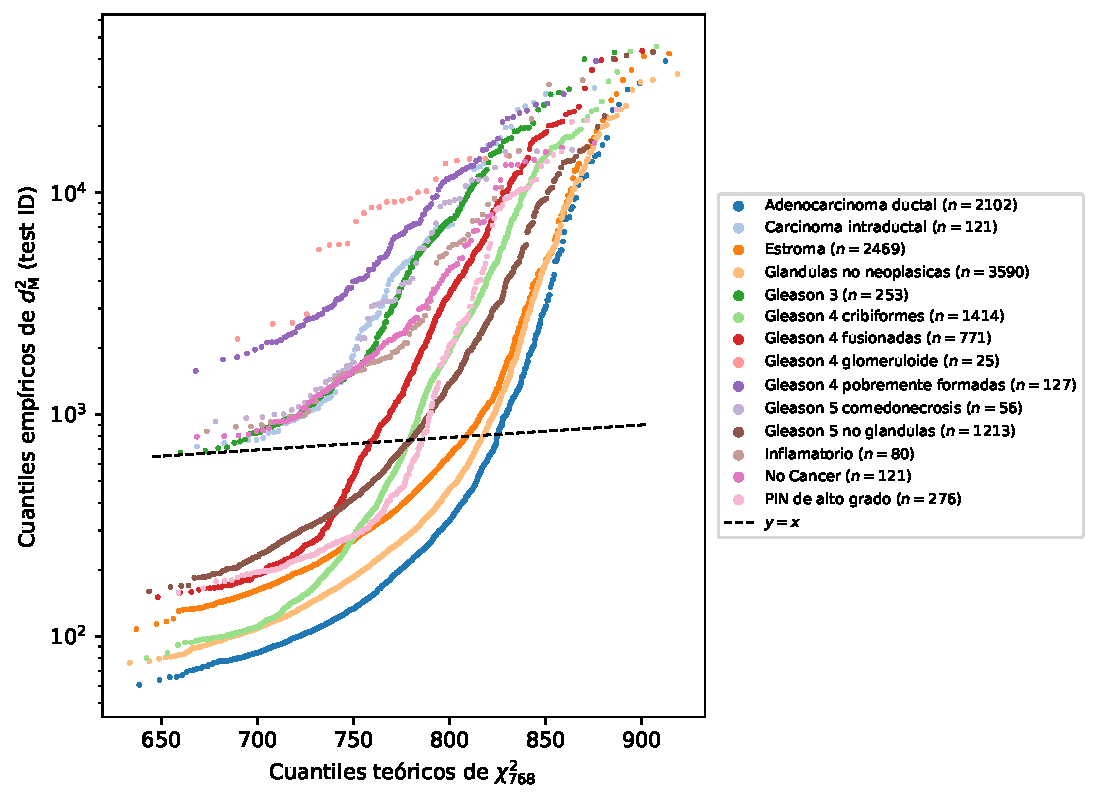
\includegraphics[width=\textwidth]{img/cap10/qq_mahalanobis_chi2.pdf}
  \caption{Q-Q plot de las distancias de Mahalanobis al cuadrado de las imágenes del test ID a su clase verdadera (eje vertical, en escala logarítmica) frente a los cuantiles de la $\chi^2_{768}$ (eje horizontal), una serie por clase, con su número de imágenes $n$. Si las clases siguieran la gaussiana que supone MDS, los puntos quedarían sobre la recta discontinua $y = x$.}
  \label{fig:ood-qq-mahalanobis}
\end{figure}

Ninguna clase queda sobre la recta $y = x$: todas las curvas se separan de ella y tienen colas mucho más pesadas que la $\chi^2_{768}$, de modo que las características no siguen la gaussiana que supone MDS. Además, las clases grandes quedan por debajo de la recta y las pequeñas muy por encima. Frente a la mediana de la $\chi^2_{768}$, 767,3, la mediana de $d^2$ es de 240,5 en \clase{Glandulas\_no\_neoplasicas} ($n = \num{3590}$) y de 175,5 en \clase{Adenocarcinoma\_ductal} ($n = \num{2102}$), pero de 9074,7 en \clase{Gleason\_4\_glomeruloide} ($n = 25$), de 5261,1 en \clase{Gleason\_4\_pobremente\_formadas} ($n = 127$) y de 3604,8 en \clase{Carcinoma\_intraductal} ($n = 121$). Esto apunta a que tampoco se cumple la hipótesis de covarianza común, que dominan las clases grandes. Aun así, MDS funciona: separar las imágenes ID de las OOD no requiere que el modelo gaussiano sea correcto.

\section{Discusión}\label{sec:ood-discusion}

% Media aritmética y desviación típica muestral (n - 1) de cada métrica sobre las ocho filas de cada método
% en results_ood/faseC_K144/tabla_principal.csv (TUM, NORM, STR, LYM, MUS, PANDA, control 128 px, DTD); se
% excluye TUM+NORM porque es la unión de TUM y NORM. Calculada a mano a partir del CSV; no la genera
% scripts/generar_tablas.py.
\begin{table}[tbp]
\centering
\footnotesize
\setlength{\tabcolsep}{4pt}
\caption{Resultado global de los 17 métodos: media $\pm$ desviación típica de \AUROC y \CCRn{5} (más alto es mejor) y de \FPRn{95} (más bajo es mejor) sobre ocho conjuntos (TUM, NORM, STR, LYM, MUS, PANDA, control de 128\,px y DTD; se excluye TUM+NORM, unión de TUM y NORM). Clase positiva: OOD. En negrita, la mejor media entre los métodos no exploratorios. $^{a}$ASH reduce la exactitud ID al 68{,}3\,\%. $^{\dagger}$Variante exploratoria ($K_c=\min(500,\lfloor n_c/2\rfloor)$). $^{\ddagger}$100\,\% de las características y $K=144$ (\cref{sec:stoodx-seleccion-k}); el resto de filas de \stoodx usan $K=500$.}
\label{tab:ood-global}
\begin{tabular}{lccc}
\toprule
Método & \AUROC $\uparrow$ & \FPRn{95} $\downarrow$ & \CCRn{5} $\uparrow$ \\
\midrule
\multicolumn{4}{@{}l}{\textit{Basados en logits}} \\
MSP & 0{,}818 $\pm$ 0{,}079 & 0{,}890 $\pm$ 0{,}063 & 0{,}108 $\pm$ 0{,}063 \\
MaxLogit & 0{,}744 $\pm$ 0{,}089 & 0{,}937 $\pm$ 0{,}049 & 0{,}061 $\pm$ 0{,}048 \\
Energy & 0{,}734 $\pm$ 0{,}092 & 0{,}938 $\pm$ 0{,}048 & 0{,}060 $\pm$ 0{,}047 \\
\midrule
\multicolumn{4}{@{}l}{\textit{Modificación de activaciones}} \\
ReAct & 0{,}770 $\pm$ 0{,}100 & 0{,}824 $\pm$ 0{,}084 & 0{,}175 $\pm$ 0{,}084 \\
ASH$^{a}$ & 0{,}491 $\pm$ 0{,}096 & 0{,}989 $\pm$ 0{,}019 & 0{,}007 $\pm$ 0{,}015 \\
DICE & 0{,}594 $\pm$ 0{,}113 & 0{,}732 $\pm$ 0{,}168 & 0{,}266 $\pm$ 0{,}166 \\
\midrule
\multicolumn{4}{@{}l}{\textit{Características y distancias}} \\
KNN & 0{,}911 $\pm$ 0{,}066 & 0{,}261 $\pm$ 0{,}130 & 0{,}738 $\pm$ 0{,}130 \\
MDS & 0{,}926 $\pm$ 0{,}064 & 0{,}250 $\pm$ 0{,}142 & 0{,}747 $\pm$ 0{,}140 \\
RMDS & 0{,}899 $\pm$ 0{,}073 & 0{,}364 $\pm$ 0{,}342 & 0{,}633 $\pm$ 0{,}340 \\
ViM & 0{,}929 $\pm$ 0{,}061 & 0{,}241 $\pm$ 0{,}139 & 0{,}756 $\pm$ 0{,}138 \\
SHE (prod.\ escalar) & 0{,}705 $\pm$ 0{,}115 & 0{,}730 $\pm$ 0{,}159 & 0{,}270 $\pm$ 0{,}159 \\
SHE (coseno) & 0{,}864 $\pm$ 0{,}095 & 0{,}446 $\pm$ 0{,}200 & 0{,}553 $\pm$ 0{,}199 \\
SHE (euclídea) & 0{,}870 $\pm$ 0{,}098 & 0{,}447 $\pm$ 0{,}206 & 0{,}552 $\pm$ 0{,}206 \\
\midrule
\multicolumn{4}{@{}l}{\textit{STOOD-X}} \\
STOOD-X (100\,\%) & 0{,}944 $\pm$ 0{,}043 & 0{,}273 $\pm$ 0{,}220 & 0{,}716 $\pm$ 0{,}212 \\
STOOD-X ($K=144$)$^{\ddagger}$ & \textbf{0{,}972} $\pm$ 0{,}023 & \textbf{0{,}120} $\pm$ 0{,}116 & \textbf{0{,}864} $\pm$ 0{,}109 \\
STOOD-X (87,5\,\%) & 0{,}943 $\pm$ 0{,}043 & 0{,}276 $\pm$ 0{,}222 & 0{,}714 $\pm$ 0{,}214 \\
STOOD-X $K_c$$^{\dagger}$ & 0{,}931 $\pm$ 0{,}064 & 0{,}247 $\pm$ 0{,}193 & 0{,}742 $\pm$ 0{,}185 \\
\bottomrule
\end{tabular}
\end{table}
\pendiente{análisis de la \cref{tab:ood-global}}
% Orden por AUROC medio: STOOD-X K=144 0,972; STOOD-X 100 % 0,944; 87,5 % 0,943; K_c 0,931; ViM 0,929;
% MDS 0,926; KNN 0,911; RMDS 0,899. Sin STOOD-X K=144, el menor FPR@95 medio es ViM (0,241) y el mayor
% CCR@FPR5 medio también ViM (0,756), aunque STOOD-X (100 %) tiene mayor AUROC medio (0,944) y la menor
% desviación de AUROC (0,043). RMDS tiene la mayor desviación de FPR@95 (0,342), por LYM (0,992) y el control de 128 px (0,821).

\textbf{Conclusión.} Ningún método domina en todas las métricas y conjuntos. ViM ofrece el mejor equilibrio global en AUROC; RMDS, el mejor comportamiento con umbrales exigentes, aunque con un fallo severo en LYM; y STOOD-X destaca en far-OOD y en varias clases de NCT-CRC, pero es el más sensible a la resolución. El hallazgo más relevante es que los mejores detectores responden sobre todo a las condiciones de adquisición, lo que condiciona su uso en un entorno multicéntrico. \revisar{conclusiones propias del Swin; con ConvNeXt-S cambian (\cref{tab:convnext-conclusiones})}
\revisar{donde dice que \stoodx «es el más sensible a la resolución», propuesta de integrar dos cosas: que es el más sensible al \emph{covariate shift} en general (corrupciones sintéticas, \cref{sec:ood-corr-deteccion}, y ConvNeXt-S, \cref{ap:convnext}), y el matiz de la \cref{sec:ood-corr-errores}: sirve como alarma de imagen alterada, pero no es el mejor para la clasificación selectiva. No se cambia el texto del autor}
\revisar{la conclusión vale para los métodos con su configuración por defecto (STOOD-X con $K = 500$). Con $K = 144$, elegido solo con datos ID, STOOD-X es el mejor en AUROC, FPR@95 y CCR@FPR5 en todos los conjuntos salvo LYM (ViM 0,969 frente a 0,966; \cref{sec:stoodx-resultados}); hay que reescribir la conclusión teniéndolo en cuenta}

% Integrar lo hallado en las secciones anteriores y enlazar con:
% - STOOD-X en detalle (\cref{cap:stoodx}); selección de K solo con ID y K = 144
%   (\cref{sec:stoodx-seleccion-k,tab:stoodx-k144-k500}).
% - Umbral con garantía de falsas alarmas (\cref{sec:conforme-ood}).
% - Efecto de la fuga por lámina en estas cifras (\cref{cap:fuga}): con KNN y MDS, el AUROC baja
%   0,02-0,07 sin la lámina de cada parche.
% - AUPR-In y AUPR-Out en el \cref{ap:aupr}; clases ADI, BACK, DEB y MUC en el \cref{ap:anexo-nct}.
% - Corrupciones sintéticas (\cref{sec:ood-corrupciones}): STOOD-X es el más sensible a la presencia de
%   covariate shift sintético (mejor AUROC en 25 de 27 celdas), pero gradúa la severidad peor que ViM y MDS
%   (CEC) y no es el mejor para la clasificación selectiva (AUROC_err, AURC); KNN, MDS y ViM son los más
%   equilibrados; los basados en logits quedan por detrás en las tres preguntas.
% Corrupciones sintéticas (\cref{sec:ood-corrupciones}), conclusiones y limitaciones:
% - STOOD-X es el detector más sensible a la presencia de covariate shift sintético: el mejor AUROC en 25
%   de 27 celdas (24 con IC sin solapar) y el mejor FPR@95 en 22 de 27 (19 con IC sin solapar).
%   - Coherente con ConvNeXt-S (\cref{ap:convnext}), donde es el primero en PANDA y en el control.
%   - Pero gradúa la severidad peor que ViM y MDS (CEC 0,128 frente a 0,106 y 0,109) y no es el mejor para
%     seleccionar qué imágenes alteradas se pueden clasificar con fiabilidad (AUROC_err, AURC), por la
%     saturación de su estadístico.
% - Los métodos de distancia (KNN, MDS, ViM) son los más equilibrados: detectan bien la alteración,
%   gradúan la severidad y separan los aciertos de los errores.
% - Los detectores basados en logits quedan claramente por detrás en las tres preguntas.
% - Robustez y detección se complementan: el aumento de datos (brillo) hace al modelo robusto a lo
%   frecuente y benigno, y la detección cubre lo que no maneja (desenfoque, artefactos).
%   Tellez et al. (2019): no está en tfg-referencias/papers/ ni en library.bib; pedírsela al autor.
% Limitaciones:
% - los parámetros de Zhang están calibrados con PCam/LocalTCT;
% - las marcas y burbujas van en una posición fija;
% - la implementación del tono está marcada como poco fiable en el código de Zhang;
% - el bootstrap es por imagen (\cref{cap:fuga});
% - el brillo estaba en el aumento de datos;
% - en STOOD-X, el orden entre imágenes saturadas lo decide un término de ~1e-8;
% - solo se ha evaluado con el Swin-S.
\pendiente{cita de Tellez et al.\ (2019), si se usa: falta el documento}
\pendiente{discusión global}

% Repetición con ConvNeXt-S en el espacio M (\cref{ap:convnext}, tabla \cref{tab:convnext-conclusiones}). Se
% mantienen: MSP > MaxLogit > Energy, ReAct/ASH/DICE por debajo de MSP, LYM ~ TUM/NORM y MDS > KNN (9 de 9).
% Dependen del modelo: el mejor método (RMDS 0,960 en TUM+NORM), el fallo de RMDS en LYM (ConvNeXt 0,938), la
% distancia PANDA > control (no se cumple en SHE coseno y euclídea) y la coincidencia PANDA/control de STOOD-X
% (ConvNeXt 0,803).
\pendiente{remisión al \cref{ap:convnext}: conclusiones que se mantienen y que dependen del modelo}

\endinput
